\documentclass[a4paper,11pt,openright,oneside]{book}
\linespread{1.5}
\usepackage{geometry}
\geometry{a4paper,top=2.5cm,bottom=3.5cm,left=3.5cm,right=3cm,heightrounded,bindingoffset=5mm,headsep=1.5cm,includehead}
\usepackage[font={small,it}]{caption}	
\usepackage[utf8]{inputenc}
\usepackage[italian]{babel} 
\usepackage{amsmath}
\usepackage[hyphens]{url}
\usepackage{graphicx}
\usepackage{fancyhdr}
\usepackage{listings}

%\usepackage[a-1b]{pdfx} %pdfa
%\hypersetup{% Personalizzazioni di hyperref
%  pdfpagemode={UseOutlines},
%  colorlinks={false},
%  hidelinks
%}
\begin{document}
\frontmatter
\begin{titlepage}
\begin{center}

{{\Large{{\bf UNIVERSIT\`A DEGLI STUDI DI MILANO}}}}
\rule[0.1cm]{13cm}{0.6mm}
{\bf Facoltà di Scienze e Tecnologie\\
Corso di Laurea Magistrale in Informatica per la Comunicazione}
\end{center}
\vspace{15mm}
\begin{center}
\vspace{3mm}
{\LARGE{\bf TECNICHE ONLINE PER L'INDIVIDUAZIONE DI SPAM IN UN WEB CRAWLER}}\\
\vspace{3mm}
\end{center}

\vspace{40mm}
\par
\noindent
\begin{minipage}[t]{0.60\textwidth}
{\large{\bf Relatore:\\
Chiar.mo Prof. Paolo BOLDI}}\\
{\large{\bf Correlatore:\\
Chiar.mo Prof. Sebastiano VIGNA}}
\end{minipage}
\hfill
\begin{minipage}[t]{0.47\textwidth}\raggedleft
{\large{\bf Tesi di Laurea di:\\
Antonio LUCA\\
matr. n. 809465}}
\end{minipage}
\vspace{50mm}
\begin{center}
{\large{\bf %inserire il numero della sessione in cui ci si laurea
Anno Accademico\\ 2013 - 2014 }}%inserire l'anno accademico a cui si è iscritti
\end{center}
\end{titlepage}
\begin{titlepage}
 \
\newpage
\end{titlepage}


\chapter*{Ringraziamenti}

\begin{flushright}

Desidero ringraziare tutti coloro che mi hanno aiutato\\ e supportato nella stesura della tesi.

Ringrazio anzitutto\\ il professore Paolo Boldi e il professore Sebastiano Vigna\\ per avermi aiutato e guidato durante tutto il lavoro di tesi.\\

Infine, ho desiderio di ringraziare le persone a me più care:\\ la mia famiglia, che mi ha sempre sostenuto,\\ e la mia fidanzata Eliana\\ che mi è sempre vicina e mi ha sempre incoraggiato.
\end{flushright}
\tableofcontents
\listoffigures
\mainmatter
\chapter{Introduzione}
\lstset{basicstyle=\small\ttfamily,keywordstyle=\color{black}\bfseries,commentstyle=\color{darkgray},stringstyle=\color{black},showstringspaces=true}

Questa tesi ha come obbiettivo lo studio e l'analisi delle tecniche di spam detection attualmente esistenti ed in particolare delle tecniche online. Nella prima parte le tecniche verranno classificate sulla base dei segnali che utilizzano. Successivamente verranno eseguiti dei test per valutare alcuni algoritmi di spam detection offline eseguiti durante la fase di crawling. Ed infine verrano presentati e discussi i risultati ottenuti. Al momento in cui si scrive non ci sono, o meglio sono poche, le tecniche online di spam detection, ovvero tecniche che rilevano lo spam durante la fase di crawling. Infatti quasi tutti i metodi tentano di fare il crawling dell'intera porzione di web di interesse e successivamente classificare le pagine in classi (dove di norma le classi sono due: \textit{spam} oppure \textit{non spam}).

Il fenomeno del web spam è sempre più presente all'interno del web: questo è dovuto al fatto che gli utenti tendono ad esaminare solo i primi risultati calcolati dai motori di ricerca e quindi se un sito fa parte degli \textit{n} primi risultati può avere un ritorno economico legato alla quantità di traffico che viene generata per quel sito. Uno studio  del 2005 descritto in \cite{Nicholas:2005} stima che la perdita finanziaria mondiale causata dallo spam e di circa 50 miliardi di dollari e nel 2009 (come descritto in \cite{Nicholas:2009}) è salita a 130 miliardi di dollari. Per questo motivo, recentemente tutte le più grandi compagnie di motori di ricerca hanno identificato il recupero di informazioni non pertinenti come una delle priorità da risolvere. Le conseguenze del web spam possono essere riassunte come segue\cite{Spirin:2012:SWS:2207243.2207252}:
\begin{itemize}
 \item la qualità delle ricerche è compromessa penalizzando i siti web legittimi;
 \item un utente potrebbe perdere la fiducia sulla qualità di un motore di ricerca e perciò passare con facilità all'utilizzo di un altro;
 \item inoltre i siti spam possono essere usati come mezzo per malware, pubblicazione di contenuto per adulti e attacchi di tipo ``fishing''. Una prova tangibile si può vedere in \cite{Eiron:2004:RWF:988672.988714}, dove gli autori hanno eseguito l'algoritmo di \textit{PageRank} su 100 milioni di pagine e hanno notato che 11 sui primi 20 risultati erano composti da siti con contenuto per adulti.
\end{itemize}
Queste considerazioni evidenziano che quando si progetta un motore di ricerca bisogna tenere conto delle pagine che potrebbero portare al mal funzionamento del motore stesso.
%questa parte forse è da cambiare in quanto il lavoro sta cambiando infatti dallo sviluppo di un modulo siamo passati a fare dei test degli algoritmi di spam
%detection su grafo
Il lavoro prodotto sarà utilizzato per essere integrato	all'interno di un web crawler distribuito ad alte prestazioni per il futuro sviluppo di un modulo di spam detection. L'esigenza di tale modulo è sorta a seguito dello sviluppo, presso il Dipartimento, di un crawler chiamato {\itshape BUbiNG}, altamente configurabile ma privo al momento di qualunque forma di rilevazione di siti e contenuti malevoli. Il problema è estremamente interessante sia dal punto di vista teorico che da quello pratico: infatti, sebbene siano numerose le tecniche descritte in letteratura per la determinazione di spam (usando come segnali sia il contenuto che la struttura dei link), è sorprendentemente scarso l'insieme di tali tecniche che possono essere usate on-line, cioè durante il crawl. Il problema diventa ancora più complesso se si aggiungono considerazioni legate ai vincoli di spazio di memoria disponibile e tempo di calcolo.
Infatti in letteratura il processo di spam detection viene eseguito subito dopo la fase di crawling. Ovvero il processo è composto dai seguenti passi:
\begin{itemize}
 \item crawling dell'intero web;
 \item fase di spam detection;
 \item indicizzazione.
\end{itemize}
Questo modello è utile perché molte delle tecniche utilizzate fanno delle analisi sul grafo che è il risultato della fine del processo di crawling. Da queste considerazioni noi proviamo a fare delle analisi per determinare se il processo di spam detection può essere fatto durante la fase di crawling ovvero al momento in cui il crawler esegue il ``fetch'' di una pagina per determinare ``on the fly'' se la pagina è buona o ha un contenuto malevolo. 

\section{Ranking dei motori di ricerca}
Prima di spiegare i vari metodi con cui si possono creare pagine web spam e successivamente quelli utili ad identificarlo, è necessario capire come i motori di ricerca sono capaci di valutare la rilevanza di una pagina web per una determinata query.
%preso dalle dispense

In linea di massima un sistema di reperimento di informazioni ovvero un motore di ricerca è dato da una collezione documentale \textit{D} (un insieme di documenti) di dimensione \textit{N} , da un insieme \textit{Q} di interrogazioni, e da funzione di ranking (\(r : Q \times D \rightarrow R\)) che
assegna a ogni coppia formata da un’interrogazione e un documento un numero reale. L’idea è che a fronte di un’interrogazione a ogni documento viene assegnato un punteggio reale: i documenti con punteggio nullo non sono considerati rilevanti, mentre quelli a punteggio non nullo sono tanto più rilevanti quanto più il punteggio è alto. In particolare i metodi di ranking si dividono in \textit{endogeni} ed \textit{esogeni}. I primi metodi fanno uso del contenuto del documento per valutarne la rilevanza mentre i secondi fanno uso di un struttura esterna ad esempio il grafo composto dai collegamenti ipertestuali tra le pagine web, questo non implica che i metodi esogeni non possono fare uso del contenuto della pagina (per esempio il testo delle ancore). I criteri si dividono ulteriormente in statici (o indipendenti dall’interrogazione) e dinamici (o dipendenti dall’interrogazione). Nel primo caso, il punteggio assegnato a ciascun documento è fisso e indipendente da un'interrogazione \textit{q} mentre nel secondo 
il punteggio assegnato a ciascun documento e dipendente da un'interrogazione \textit{q}.

Tra i metodi endogeni sono di maggiore importanza \textit{tf-idf} e \textit{BM25} mentre tra quelli esogeni i più diffusi in letteratura sono \textit{PageRank} e \textit{HITS}.

\subsection{Metodi di ranking endogeno}
Come già detto i precedenza i metodi di ranking endogeno utilizzano il contenuto di una pagina per assegnarle un punteggio. Possono essere anch’essi statici o dinamici (cioè dipendere o meno da un’interrogazione). L'algoritmo usato dai motori di ricerca per fare il rank delle pagine web basandosi sui campi di testo usa varie forme del \textit{tf-idf}. Il \textit{tf-idf} e un metodo di ranking endogeno dinamico che utilizza il contenuto di una pagina per assegnarle un punteggio. Il \textit{tf-idf} è una misura composta da due misure più semplici: la \textit{Term Frequency} e la \textit{Inverse Document Frequency}. Il primo metodo assegna a un documento \textit{d} il punteggio dato dalla somma dei conteggi dei termini \textit{t} dell'interrogazione che compaiono nel documento stesso. In questo modo documenti in cui i termini dell'interrogazione compaiono più frequentemente avranno un punteggio più elevato. Utilizzare solo questo metodo non conviene in quanto è facilmente manipolabile. Inoltre non tiene conto 
del fatto che alcuni termini occorrono più frequentemente non perché rilevanti, ma perché altamente frequenti all'interno di \textit{ogni} documento (ad esempio le congiunzioni). Il secondo metodo è definito come l'inverso del numero di documenti nella collezione che contengono il termine \textit{t} \cite{Manning:2008:IIR:1394399p117}. Più precisamente:
\begin{equation}
 idf_t=\log\frac{N}{df_t}
 \label{eq:idf}
\end{equation}
La combinazione del \textit{tf} ed dell'\textit{idf} produce una misura composta che permette di normalizzare il peso dei termini. Il \textit{tf-idf} di un documento \textit{d} rispetto a una query \textit{q} è calcolato su tutti i termini \textit{t} in comune come:
\begin{equation}
 tf-idf(d,q)=\sum_{t \in d \: and \: t \in q} tf(t,d) \cdot idf(t)
\end{equation}
Con il \textit{tf-idf} gli spammer possono avere due obbiettivi: o creare pagine rilevanti per un gran numero di query o creare pagine molto rilevanti per una specifica query. Il primo obbiettivo può essere ottenuto includendo un gran numero di termini distinti in un documento; il secondo, attraverso la ripetizione di determinati termini nel documento.

Un altro metodo di ranking endogeno dinamico è \textit{BM25} \cite{Robertson:2009:PRF:1704809.1704810} che è uno schema di pesatura basato sul \textit{modello probabilistico} ed attualmente è il sistema di pesatura più usato. 

\subsection{Metodi di ranking esogeno}
Uno dei metodi esogeni statici è \textit{PageRank} descritto in \cite{ilprints422}. PageRank usa le informazioni portate dai link in entrata (\textit{inlink}) per determinare un punteggio globale di importanza di una pagina. Esso assume che esista un legame tra il numero di \textit{inlink} di una pagina \textit{p} e la popolarità della pagina \textit{p}. Il concetto fondamentale dietro \textit{PageRank} è che una pagina è importante se molte altre pagine importanti puntano ad essa. Questo concetto è mutualmente rinforzante ovvero l'importanza di una certa pagina influenza ed è influenzata dall'importanza delle altre pagine \cite{ilprints646}. In dettaglio \textit{PageRank} è basato sulla passeggiata naturale del grafo del web \textit{G}. Più precisamente, la passeggiata viene perturbata nel seguente modo: fissato un parametro \(\alpha\) tra \(0\) e \(1\), a ogni passo con probabilità \(\alpha\) si segue un arco uscente, e con probabilità \(1- \alpha \) si sceglie un qualunque altro nodo del grafo utilizzando 
una 
qualche 
distribuzione \(v\), detta
vettore di preferenza (per esempio, uniforme). Assumendo che non esistano pozzi, la matrice di transizione della catena è quindi rappresentata dalla combinazione lineare:
\begin{equation}
 \alpha G + (1 - \alpha) 1 v^T
\end{equation}
dove \(G\) è la matrice della passeggiata naturale su \(G\). Il fattore \(\alpha\) è detto fattore di attenuazione di norma è impostato a un valore di 0,85.

Un altro metodo esogeno usato per il ranking delle pagine è \textit{HITS (Hyperlink Induced Topic Distillation)} introdotto in \cite{Kleinberg:1999:ASH:324133.324140}. Differentemente da \textit{PageRank} esso assegna due punteggi di importanza a ogni pagina: uno di \textit{hubbines} e uno di \textit{autorevolezza}. L’intuizione dietro a HITS è che invece di un singolo punteggio di importanza esista un concetto di pagina \textit{autorevole}, cioè pagina con contenuto pertinente e interessante, e di \textit{hub}, cioè pagina contenente numerosi collegamenti a pagine autorevoli. I due concetti si rinforzano \textit{mutuamente}: una pagina autorevole è puntata da molte pagine centrali, e una buona pagina centrale punta a molte pagine autorevoli.

Questo approccio considera che nel web ci sono due tipi di pagine: quelle che contengono dei contenuti per un determinato argomento (\textit{authoritative}) e quelle che contengono tanti link a delle pagine \textit{authoritative} che sono chiamate pagine \textit{hub}. Le pagine \textit{hub} sono utili per scoprire le pagine \textit{authoritative} \cite{Manning:2008:IIR:1394399p474}.

L'algoritmo lavora su un sottografo del web ottenuto a partire da un'interrogazione. La selezione del sottografo può essere fatta in vari modi, un modo è quello di prendere un certo insieme di risultati  ottenuto da un motore di base e generare un sottografo sulla base di una query e delle pagine che puntano a quelle ottenute dalla query. Per questo sottoinsieme di pagine otteniamo un matrice di adiacenza \(A\). I punteggi di \textit{hub} e \textit{authority} per tutte le pagine del sottoinsieme possono essere formalizzate dalla seguente coppia di equazioni:
\begin{equation}
 \left\{
 \begin{array}{cc}
    \stackrel{\rightarrow}{a_{t+1}} \: = \: A^T \stackrel{\rightarrow}{h_t}\\
    \stackrel{\rightarrow}{h_{t+1}} \:= A \: \stackrel{\rightarrow}{a_{t+1}}
 \end{array}
 \right .
 \label{eq:hubat}
\end{equation}
Può essere dimostrato che la soluzione ottenuta applicando iterativamente il sistema \ref{eq:hubat} converge rispettivamente al principale autovettore di \(AA^T\) e \(A^TA\) \cite{Manning:2008:IIR:1394399p474}\cite{Spirin:2012:SWS:2207243.2207252}.

\section{Web spam}
Con il termine web spamming si fa riferimento a tutti i metodi che tentano di manipolare gli algoritmi di ranking dei motori di ricerca per aumentare il valore di alcune pagine rispetto ad altre \cite{ilprints646}.
Dato il numero esorbitante di pagine che vengono create e pubblicate sul web, gli utenti competono per far comparire le proprie pagine tra le prime dei risultati di una query.
Il fenomeno dello spamming o spamindexing ricade sulla qualità delle ricerche causando diversi problemi: indicizzazione di pagine che non sono utili, aumento del costo delle operazioni di query, malware e reindirizzamento verso contenuto per adulti; inoltre questo spinge gli utenti ad utilizzare altri motori di ricerca \cite{Spirin:2012:SWS:2207243.2207252}.

L'obbiettivo del motori di ricerca è di ottenere ottimi risultati per identificare tutte le pagine web che sono rilevanti per una specifica query e presentarle secondo l'importanza che esse hanno. Di norma la rilevanza viene misurata attraverso la similarità testuale tra la query e le pagine mentre l'importanza è definita come la popolarità globale della pagina e a volte è inferita dalla struttura dei link \cite{ilprints646}. Ci sono due categorie di tecniche associate al web spam \cite{ilprints646}:
\begin{itemize}
\item \textbf{tecniche boost} che cercano di far avere più importanza o rilevanza a delle pagine
\item \textbf{tecniche hiding} che sono metodi per nascondere le tecniche di boost all'utente dal browser, anche se alcuni autori incorporano queste tecniche fra quelle di boost.
\end{itemize}

\subsection{Tecniche di boost}
Le tecniche di boosting si dividono in: \textit{Term Spamming} e \textit{Link Spamming}. Con l'avvento degli algoritmi di ranking basati sulla struttura del grafo il \textit{Term Spaming} è stato trascurato. In figura \ref{fig:tassonomiaTecnicheBoost} è specificata una possibile tassonomia delle tecniche boost \cite{ilprints646}.
\begin{figure} 
 \centering
 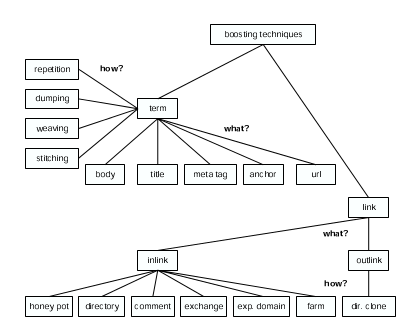
\includegraphics[width=12cm]{immagini/tassonomiaTecnicheBoost}
 \caption{Tassonomia delle tecniche boost}
 \label{fig:tassonomiaTecnicheBoost}
\end{figure}

\subsection{Term Spamming}
Nel valutare la rilevanza testuale i motori di ricerca considerano dove i termini di una query compaiono in una pagina. Il tipo di punto all'interno della pagina è chiamato \textit{campo}. I più comuni campi di testo per una pagina \textit{p} sono: il body della pagina, il titolo, i meta tag nell'header HTML e l'URL della pagina. Inoltre viene considerato anche come \textit{campo}, il testo delle ancore (il tag \textit{a}) associate all'URL che puntano alla pagina \textit{p} dato che descrive molto bene il contenuto della pagina . I campi di testo  di \textit{p} sono utilizzati per determinare la rilevanza di \textit{p} rispetto ad una query (alcune volte i campi vengono pesati sulla base della loro importanza) e perciò chi fa \textit{term spamming} utilizza tecniche di pesatura dei contenuti dei campi di testo in modo tale da aumentare l'efficacia dello spam \cite{ilprints646}. Le tecniche di spamming possono essere raggruppate in base ai \textit{campi} di testo dove viene fatto spamming. In base a 
questo distinguiamo \cite{ilprints646}:
\begin{itemize}
\item \textit{Body Spam}. In questo caso lo spam è nel corpo del documento. Questo è lo spam più diffuso.
\item \textit{Title Spam}. Molti motori di ricerca danno molta importanza ai termini che compaiono nel titolo. Quindi ha senso includere termini di spam all'interno del titolo della pagina.
\item \textit{Meta Tag Spam}. I tag che compaiono nell'header sono molto frequentemente soggetti a spam. Per questo i motori di ricerca danno poca importanza a questi campi o non li considerano. Di seguito viene mostrato un esempio di questo tipo di spam.
\begin{lstlisting}[frame=trbl,postbreak=\space, breakindent=5pt, breaklines]
 <meta name="keyword" content="buy, cheap, cameras, lens, accessories, nikon, canon">
\end{lstlisting}
\item \textit{Anchor Text Spam}. I motori di ricerca assegnano un peso maggiore al testo nelle ancore perché pensano che esse contengano un riassunto del contenuto della pagina. Perciò del testo di spam è incluso nel testo delle ancore dei collegamenti HTML di una pagina. In questo caso lo spamming non viene fatto sulla pagina cui si vuole far avere un rank più alto ma sulle pagine che puntano ad essa.
\begin{lstlisting}[frame=trbl,postbreak=\space, breakindent=5pt, breaklines]
<a href="target.html">free, great deals, cheap, inexpensive, cheap, free</a>
\end{lstlisting}
\item \textit{URL Spam}. Alcuni motori di ricerca dividono l'URL delle pagine in un insieme di termini che sono usati per determinare la rilevanza di una pagina. Per sfruttare questo metodo di ranking, gli spammer creano lunghi URL che includono una grande sequenza di termini spam, un esempio può essere: \textit{buy-canon-rebel-20d-lens-case.camerasx.com}.
\end{itemize}
Queste tecniche possono essere utilizzate insieme o separatamente. Un altro modo per raggruppare queste tecniche si basa sul tipo di termini che vengono utilizzati nei campi di testo \cite{ilprints646}, possiamo avere:
\begin{itemize}
\item Ripetizione di uno o più specifici termini.
\item Inclusione di molti termini generici per creare pagine rilevanti per molte query.
\item Intreccio di vari termini all'interno della pagina.
\item Creazione di frasi di senso compiuto per l'elaborazione di contenuti generati velocemente attraverso la concatenazione di frasi da fonti diverse.
\end{itemize}

\subsection{Link Spamming}
Il \textit{link spamming} è un tipo di spam che fa uso della struttura dei link tra le pagine web per favorire il rank di una pagina target \textit{t}.
In \cite{ilprints646} si afferma che per uno spammer ci sono tre tipi di pagine nel Web: inaccessibili, accessibili(blog) e proprietarie (fig. \ref{fig:tipologiaPagine}). Le inaccessibili sono quelle che uno spammer non può modificare. Le accessibili sono pagine gestite da altri ma che possono essere modificate lievemente dallo spammer attraverso l'immissione di un post in un forum o in un blog o portali di questo genere. Le proprietarie sono pagine su cui gli spammer hanno il pieno controllo. Il gruppo di pagine proprietarie è chiamato \textit{spam farm}.
\begin{figure} 
 \centering
 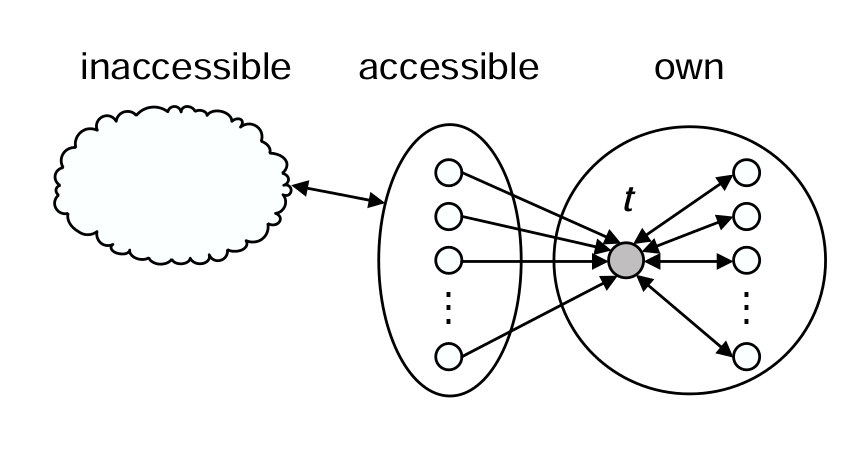
\includegraphics[width=10cm]{immagini/tipologiaPagine}
 \caption{Tipi di pagine nel web per uno spammer}
 \label{fig:tipologiaPagine}
\end{figure}

Molti motori di ricerca utilizzano due algoritmi per aumentare l'importanza basandosi sulle informazioni dei link: PageRank e HITS; sulla base di questi due tipi di algoritmi vengono definite due categorie principali di \textit{link spamming}: \textit{outgoing link spam} e \textit{incomign link spam}. L'\textit{outgoing link} è uno dei metodi più facili da implementare in quanto basta aggiungere dei link nella propria pagina, ad altre pagine che sono considerate buone, sperando di poter aumentare il  punteggio di \textit{hub}. Per la ricerca di link da includere nella pagina per cui si vuole incrementare il punteggio di \textit{hub} si possono utilizzare delle directory che contengono liste di siti come DMOZ o Yahoo!. Queste directory organizzano i contenuti web in contenuti e in liste di siti relativi. Per quanto riguarda \textit{incoming link}, ci sono diverse strategie che si possono adottare in modo tale da avere un numero elevato di link in entrata \cite{ilprints646}:
\begin{itemize}
\item \textit{Honeypot}: ovvero si creano un insieme di pagine che hanno un contenuto interessante (un esempio può essere una documentazione Linux) ma che hanno link nascosti alla pagina o alle pagine per cui si deve aumentare il valore di rilevanza.  
\item \textit{Infiltrarsi in una directory web}: molte directory web permettono ai webmasters di postare link ai loro siti che hanno lo stesso contenuto.
\item \textit{Postare link nei blog, forum e wiki}: includere URL a pagine di spam come parte di un commento.
\item \textit{Scambio di link}: scambiare link con altre pagine di spam. Questa è una pratica comune tra chi fa spam ed esistono blog completamente finalizzati all'incontro di spammer per lo scambio dei link.
\item \textit{Comprare domini scaduti}: quando un dominio scade ci sono delle pagine che puntano ancora ad esso. Una tecnica è comprare questi domini e manipolare le pagine in modo tale da fare aumentare il rank di una pagina target.
\item \textit{Creare una spam farm}: con l'abbassamento dei costi si possono costruire delle spam farm che hanno come obbiettivo di aumentare la rilevanza di un pagina spam detta \textit{target page}, un esempio è mostrato in fig. \ref{fig:spamfarm}. Molte volte si utilizzano tecniche come \textit{honeypot}. In questo caso il valore di page rank aggregato delle pagine è propagato alla pagina target. Una delle forme più aggressive di honeypot è l'\textit{hijacking} \cite{Spirin:2012:SWS:2207243.2207252}, dove gli spammer prima attaccano un sito con una buona reputabilità e poi usano questo come parte della loro link farm.
\end{itemize}
\begin{figure} 
 \centering
 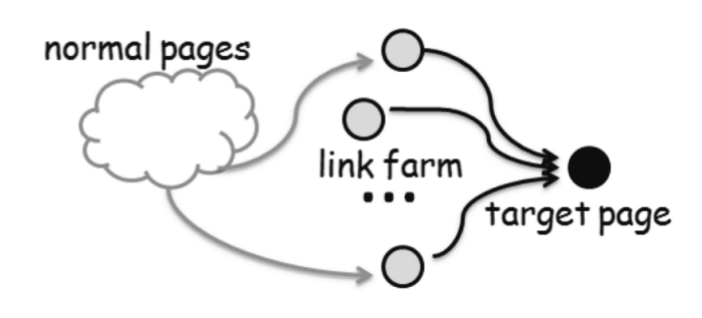
\includegraphics[width=10cm]{immagini/spamfarm}
 \caption{Esempio di una spamfarm}
 \label{fig:spamfarm}
\end{figure}

\subsection{Tecniche di hiding}
Le tecniche di hiding si possono classificare in: \textit{content hiding}, \textit{cloaking}, \textit{redirection} (fig. \ref{fig:tecnicheHiding}) \cite{ilprints646}.
\begin{figure} 
 \centering
 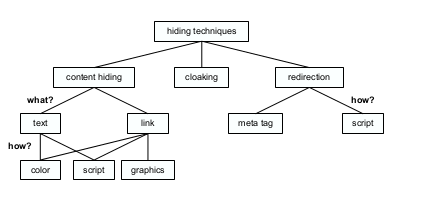
\includegraphics[width=10cm]{immagini/tassonomiaHiding}
 \caption{Tecniche di hiding}
 \label{fig:tecnicheHiding}
\end{figure}
Nel \textit{Content hiding} i termini o link di spam possono essere nascosti quando il browser visualizza una pagina. Una tecnica è quella di utilizzare lo stesso colore per i termini e lo sfondo. Mentre per i link basta non inserire il testo all'interno delle ancore che indirizzano a una pagina. Un'altra tecnica è quella di utilizzare degli script per nascondere il contenuto. Il \textit{Cloaking} sfrutta il fatto che è facile identificare quando la richiesta di una pagina è fatta da un crawler o da un browser: questa tecnica dato un URL, il server spam restituisce un documento HTML diverso a seconda che la richiesta sia fatta da un crawler o da un browser. Quindi vengono distribuiti due contenuti diversi in base al fatto che la richiesta al server spam sia fatta da un crawler o da un browser. La rilevazione di un crawler può essere effettuata in due modi: o si mantiene in memoria una lista di indirizzi di crawler oppure si usa l'header della richiesta HTTP andando a vedere il campo user-agent: se questo è 
diverso dai 
più comuni browser allora può essere un crawler. Nell'esempio sotto, lo user-agent della richiesta HTML indica l'uso del web browser Chrome.
\begin{lstlisting}[frame=trbl,postbreak=\space, breakindent=5pt, breaklines]
Mozilla/5.0 (X11; Linux x86_64) 
AppleWebKit/537.36 (KHTML, like Gecko) 
Chrome/32.0.1700.102 Safari/537.36
\end{lstlisting}
La \textit{Redirection} è un'altra tecnica che reindirizza il browser ad un altro URL appena la pagina è caricata. Un esempio di redirection server-side è mostrato di seguito.
\begin{lstlisting}[frame=trbl,postbreak=\space, breakindent=5pt, breaklines]
header("Location: http://www.example.com/");
\end{lstlisting}
\subsection{Click Spamming}
Un ultimo metodo per fare web spam è il \textit{Click Spamming} \cite{Spirin:2012:SWS:2207243.2207252}. I motori di ricerca utilizzano dati sul flusso dei click per regolare le funzioni di ranking, quindi  gli spammer generano clik fraudolenti per manipolare il comportamento di queste funzioni in modo tale da fare avere un rank migliore ai loro siti. Il metodo prevede che vengano fatte delle query e si clicchi sulla pagina di cui si vuole aumentare il rank. Tale metodo viene eseguito in modo automatico attraverso script che girano su diverse macchine per non fare sospettare il motore di ricerca delle numerose richieste provenienti da un unica macchina \cite{Spirin:2012:SWS:2207243.2207252}.



\chapter{Tecniche di spam detection}
Il capitolo illustra le tecniche per spam detection presenti in letteratura al momento in cui si sta scrivendo. Le tecniche verrano divise sulla base del tipo di segnali che usano: contenuto, grafo ottenuto dalla fase di crawling, altri segnali (es. header delle richieste HTTP). Nella prima parte del capitolo verranno illustrate le tecniche basate sul contenuto, nella parta centrale le tecniche basate su grafo ed infine le tecniche che fanno uso di altri tipi di segnali.

\section{Tecniche basate sul contenuto}
Uno dei primi studi sul web spam è descritto in \cite{Fetterly:2004:SDS:1017074.1017077}, in questo articolo vengono eseguite delle analisi statistiche che dimostrano che le  pagine spam  hanno proprietà diverse rispetto alle pagine con contenuti. Queste proprietà sono classificate come segue:
\begin{itemize}
 \item 	Proprietà degli URL: il link spam è una particolare forma di spam dove gli spammer cercano di aumentare il rank derivato da algoritmi basati sulla struttura dei link. Uno spammer cerca di creare automaticamente delle pagine di bassa qualità che puntano a una pagina target \textit{p}. In questo articolo viene fatta un'analisi sulle proprietà dei link ed è stato trovato che le caratteristiche degli URL di un HOST sono indizzi per identificare lo spam. In particolare è stato trovato che il nome di un HOST con molti caratteri, punti, barre e numeri è un buon indicatore di spam. Un modo semplice per classificare le pagine sarebbe quello di usare un soglia. % immagine grafico
 \item Host name resolution: Alcuni motori di ricerca (Google) data una query q, danno un rank più alto a un URL u se i componenti dell'host di u conentengo i termini della query. Gli spammers per sfruttare questo popolano le pagine con le URL le cui componenti contengono query popolari che sono rilevanti per un certo settore e impostano un DNS per risolvere questi host name. Spammers creano un grande numero di nomi per avere un alto rank per una grande varietà di query. Per determinare questa forma di spam basta vedere quanti nomi vengono risolti con lo stesso indirizzo.


Una altra caratteristica è che Google nella sua variante di PageRank assegna un peso maggiore a link esterni e sempre di più se ci sono molti link che puntano a differenti pagine di un altro server. Spammer cercano di popolare le pagine con molti link ad altri host tipicamente questi risolvono uno o pochi indirizzi. Per rilevare lo spam in viene calcolato la media dell' host-machine-ratio. L'host-machine-ratio di una pagina è definita come la grandezza degli host name riferiti dai link all'interno della pagina diviso per la dimensione dell'insieme degli indirizzi distinti con cui gli host name vengono risolti. L'host-machine-ratio è la media degli host-machine-ratio di tutte le pagine di un host. Un host-machine-ratio alto indica che questa ci sono molti riferimenti a host differenti è questa è un indicazione di spam.
 \item Proprietà del contenuto: le pagine generate automaticamente hanno tutte lo stesso template, in particolare ci sono numerosi siti di spam che dinamicamente generano pagine che hanno uno stesso numero di parole.
 \item Proprietà clustering: una tecninca per determinare lo spam è quella di clusterizzare le pagine in base alla somiglianza dei template. Visto che le pagine di spam sono molto simili tra loro, identiicando molte pagine con la stessa struttura è probabile che siano di spam.
\end{itemize}

\chapter{Tecniche basate sul grafo}
\lstset{basicstyle=\small\ttfamily,keywordstyle=\color{black}\bfseries,commentstyle=\color{darkgray},stringstyle=\color{black},showstringspaces=true}
In questo capitolo verrano presentate le tecniche di spam detection presenti in letteratura, denominate \textit{linked base}, che si avvalgono cioè del grafo del web  derivato dalla fase di crawling, che si ricava dai collegamenti ipertesuali tra le pagine. Il web può essere rappresentato come un grafo orientato \textit{G = (V,E)} dove \textit{V} è l'insieme dei nodi del grafo e rappresenta le pagine web, ed \textit{E} è l'insieme degli archi  orientati tra i nodi e rappresenta l'insieme dei link orientati tra le pagine; assumendo che ci siano due pagine web \(a_p\) e \(b_p\) queste saranno rappresentate da due nodi del grafo \(a\) e \(b\); se esiste un collegamento ipertestuale  dalla pagina \(a_p\) alla pagina \(b_p\) allora vi sarà un arco diretto dal nodo \(a\) al nodo \(b\). 

Ogni pagina ha:
\begin{itemize}
 \item  link in uscita (\textit{outlink}) ovvero i link presenti nella pagina che referenziano altre pagine web;
 \item  link in entrata (\textit{inlink}) ovvero tutti i riferimenti della pagina fatti da altre pagine.
\end{itemize}

Il grafo del web può essere astratto e rappresentato da una matrice di transizione cosi formata:
\begin{equation}
T(p,q)=\left \{
\begin{array}{cc}
0 & if(p,q) \not\in E\\
1/\omega(p) & if(p,q) \in E
\end{array}
\right .
\end{equation}
dove \(q\) e \(p\) sono delle pagine web appartenenti al grafo e \(\omega(p)\) è il grado di link in uscita della pagina \(p\). 
Possiamo anche definire la matrice di transizione inversa U:
\begin{equation}
U(p,q)=\left \{
\begin{array}{cc}
0 & if(q,p) \not\in E\\
1/l(p) & if(q,p) \in E
\end{array}
\right .
\end{equation}
dove \(l(p)\) è il grado di link in ingresso della pagina \(p\). Bisogna notare che \(U \not = T^T\), ovvero la matrice di transizione inversa \(U\) non è uguale alla matrice di transizione trasposta.
\section{Metodi classici per identificare lo spam web usando il grafo}
Uno dei primi metodi adottati di spam detection che utilizza il grafo del web è \textit{Trustrank} \cite{Gyongyi:2004:CWS:1316689.1316740}. \textit{Trustrank} applica a un insieme di pagine di partenza \(S\) (detto anche seedset) una funzione \textit{Oracle} per classificare il seedset in due sottoinsiemi, pagine non spam \(S^+\) e pagine spam \(S^-\); tale classificazione è effettuata manualmente da esperti. Per determinare le pagine non spam senza invocare la funzione \textit{Oracle} su tutto il grafo derivato dalla fase di crawling, viene fatta un'assunzione empirica chiamata \textit{isolazione approssimata dell'insieme delle pagine buone}, la quale afferma che le pagine non spam raramente punteranno a delle pagine spam. Razionale di tale assunzione è che gli sviluppatori di pagine web non spam non hanno interesse nel linkare pagine spam (a meno che  tramite l'uso di tecniche come l'\textit{honeypot} vengano ``ingannati''). Quindi fissato un numero limitato di chiamate della funzione \textit{Oracle} sul 
seedset di partenza e sfruttando l'assunzione fatta precedentemente viene definita una funzione, denominata \textit{funzione di verità ignorante \(T_0\)}, per ogni pagina pagina \(p\) del grafo:
\begin{equation}
T_0(p)=\left\{
\begin{array}{ccc}
O(p) & if & p\in S \\
1/2 & altrimenti
\end{array}
\right .
\end{equation}
dove la funzione \(O\) è la funzione \textit{Oracle}. Presupponendo che le pagine non spam puntino ad altre pagine non spam viene assegnato il valore 1 a tutte le pagine che possono essere raggiunte da una pagina in \(S^+\) in \(M\) step. La funzione di verità \(T_M\) è definita come:
\begin{equation}
T_M(p)=\left\{
\begin{array}{ccccc}
O(p) & if & p\in S \\
1 & if & p \not\in S & and & \exists q\in S^+:q\rightarrow_M p \\
1/2 & altrimenti
\end{array}
\right .
\end{equation}
Il percorso  dalla pagina \(q\) a \(p\) nell'equazione non comprende pagine spam incluse nell'insieme \(S^-\).
\begin{figure}
\centering
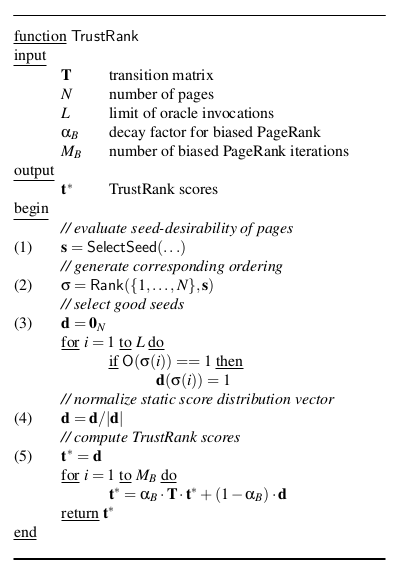
\includegraphics[width=8cm]{immagini/trustrank/trustrank}
\caption{Algoritmo di trustrank}
\label{fig:trustrank1}
\end{figure}
Limite della funzione di verità \(T_M\) è che si basa su un'euristica, quindi non esiste la sicurezza che le pagine raggiungibili da pagine non spam siano effettivamente della pagine non spam; tale sicurezza si riduce quanto più lontana dal seedset \(S^+\) è una pagina \(p\). Per non incorrere in tale errore si può ridurre il valore della funzione di verità in maniera proporzionale alla distanza dal seedset \(S^+\).

In figura \ref{fig:trustrank1} è illustrato lo pseudo-codice dell'algoritmo di \textit{Trustrank}; sarà descritto in dettaglio come funziona. 

I valori di input dell'algoritmo sono:
\begin{itemize}
 \item il grafo descritto dalla matrice di transizione \(T\);
 \item il numero di pagine \(N\);
 \item i parametri di controllo dell'esecuzione: \(L\) è il numero di chiamate della funzione \(Oracle\), \(\alpha_b\) è il fattore di decadimento per il calcolo di \textit{PageRank} ed infine \(M_b\) è il numero di iterazioni per il calcolo di \textit{PageRank}.
\end{itemize}

Al primo passo viene invocata la funzione \textit{SelectSeed()} che calcola l'insieme delle pagine con un relativo punteggio di pertinenza da includere nel seedset di partenza. Gli autori consigliano due metodi per implementare questa funzione : 
\begin{itemize}
 \item il primo metodo, chiamato \textit{Inverse PageRank}, attribuisce una preferenza alle pagine dalle quali si possono raggiungere molte altre pagine,  applicando l'algoritmo di PageRank sul grafo trasposto;
\item il secondo metodo, detto \textit{High PageRank}, assegna un alto valore di pertinenza a pagine che hanno un alto valore di pagerank.
\end{itemize}

Nell'istruzione (2) della figura \ref{fig:trustrank1} la funzione \(Rank(x,s)\) ordina gli elementi di \(x\) in modo decrescente sulla base dello score di \(s\). 

Nel punto (3) della figura \ref{fig:trustrank1} invoca la funzione \textit{Oracle} su \(L\) pagine, impostando a 1 i valori del vettore \(d\) che rappresenta l'insieme delle pagine del seedset.

Nel punto (4), ai valori del vettore \(d\), viene applicata una normalizzazione in modo tale che la somma faccia 1. 

Infine al punto (5) viene calcolato \textit{Trustrank} usando \textit{Pagerank} dove il vettore di teletrasporto è rimpiazzato dal vettore \(d\). Dall'algoritmo si nota che \textit{Trustrank} è una versione personalizzata di \textit{Pagerank} dove il vettore di teletrasporto è il seedset \(S^+\) calcolato al punto 3 e 4. L'obbiettivo è quindi assegnare un valore di verità alto alle pagine non spam e basso per le pagine spam.


Un altro algoritmo progettato per identificare lo spam usando come input il grafo delle pagine web è \textit{Anti-Trust Rank} \cite{Krishnan06webspam}. Partendo dalla stessa intuizione dell'isolamento approssimato ovvero che pagine non spam molto raramente puntino a pagine malevoli, \textit{Anti-trust rank}  popola un seedset formato da pagine spam e propaga la funzione Antitrust (corrispondente alla funzione di verità di Trustrank) sul grafo trasposto con l’obbiettivo di rilevare le pagine spam, che potranno quindi essere filtrate da un motore di ricerca. Più precisamente, a differenza di quanto avviene in \textit{Trustrank} dove la funzione \textit{Trust} è propagata dal seedset composto da pagine non spam lungo tutto il grafo, in \textit{Anti-Trust Rank} la funzione \textit{Anti Trust} è propagata nella direzione inversa ai link in entrata ad ogni pagina del grafo, partendo da un insieme di pagine del seedset composto da pagine spam. L'obbiettivo è assegnare un rank maggiore alle pagine spam e 
successivamente eliminarle dalle ricerche impostando un valore soglia tramite il quale escluderle oppure restituendo le \(n\) pagine che hanno valore di \textit{Anti-Trust Rank} più alto.
 
\textit{Trustrank} e \textit{Anti-Trust rank} sono ottimi algoritmi per identificare lo spam ma hanno il problema relativo alla dimensione dell’insieme  seedset, in quanto tale seedset potrebbe non essere sufficientemente rappresentativo per campionare tutti gli argomenti del web. Per tentare di risolvere questo problema è stato implementato un metodo \cite{Wu:2006:TTU:1135777.1135792}  che fa uso degli argomenti delle pagine come segnale di ingresso;  invece di usare un singolo valore di \textit{trustrank} per un nodo, vengono estrapolati per ogni pagina gli argomenti contenuti. L'algoritmo partiziona il seedset sulla base dei vari argomenti che esso contiene e usa ognuna di queste partizioni come seedset di partenza per calcolare il valore di \textit{trustrank} per ogni pagina.

 In letteratura viene descritto un metodo di spam detection  \cite{Caverlee:2007:CWS:1281100.1281124} \textit{linked base} che è difficilmente manipolabile tramite tecniche come \textit{honeypot}, a differenza dei precedenti metodi illustrati in questo capitolo . Infatti tale metodo separa la credibilità di una pagina dalla credibilità del link per quella pagina. La credibilità viene definita in termini di credibilità \textit{k-scope}. Sia una funzione \(C\) una funzione di credibilità che istantaneamente valuta la qualità di un link di un pagina \(p\) al tempo \(t\), per valori di \(C(p,t)=0\) la funzione indica che \(p\) non è credibile mentre per  \(C(p,t)=1\) la funzione indica che \(p\) è credibile. Sia un percorso in un grafo diretto \(G\) dalla pagina \(p\) alla pagina \(q\) la sequenza di nodi: \(path(p,q)=(n_0,n_1,...,n_j)\) dove \(p=n_0, q=n_j\) tale che esista un arco diretto tra nodi successivi nel percorso \(n_i,n_{i+1}\in L\) per \(0\leq i \leq j-1\), si definisce \textit{bad path} quel 
percorso  in un grafo  diretto \(G\)  dalla pagina \(p\) alla pagina \(q\) se la pagina di destinazione è una pagina spam \(q\in P_b\) (dove \(P_b\) è l'insieme delle pagine spam) e nessuna altra pagina nel percorso è una pagina spam ovvero \(path(p,q)=(n_0,n_1,...,n_j)\) e \(q\in P_b\) e \(n_i\not\in P_b (0\leq i\leq j-1)\). La probabilità che una camminata casuale passi attraverso un percorso di lunghezza \(k\) da una pagina \(p\) è denotata con \(Pr(path_k(p))\) ed è determinata con i pesi degli archi per ogni hop nel percorso:
\begin{equation}
 PR(path_k(p))=\prod_{i=0}^{k-1}w(n,n_{i+1})
\end{equation}
Quindi la credibilità \textit{k-scope} di una pagina  è definita in termini di probabilità che una camminata casuale eviti le pagine spam dopo aver superato \(k\) hop dalla pagina di origine. La credibilità \textit{k-scope} di una pagina \(p\) al tempo \(t\), denotata con \(C_k(p,t)\), è definita come segue:
\begin{equation}
 C_k(p,t)=1-\sum_{l=1}^k\left (\sum_{path_l(p)\in BPath_l(p)}Pr(path_l(p))\right )
\end{equation}
Dove \(BPath_l(p)\) è l'insieme di tutti i \textit{bad path} di lunghezza \(l\) che hanno origine dalla pagina \(p\). Appare chiaro che nel caso in cui \(p\in P_b\) allora la credibilità \textit{k-scope} è uguale a \(C_k(p,t)=0\). Se non ci siano pagine spam all'interno di \(k\) hop  allora la pagina \(p\) è credibile con un valore \(C_k(p,t)=1\). Il metodo descritto presenta tuttavia due criticità:
\begin{itemize}
 \item è difficile costruire un grafo che rappresenti interamente tutto il web;
 \item non si conoscono tutti i nodi spam.
\end{itemize}
 Per risolvere tali criticità è stato introdotto il concetto di \textit{tunable k-scope},  il quale modifica il calcolo della credibilità k-scope includendo un fattore di penalità di credibilità. Gli obbiettivi sono approssimare al meglio la credibilità \textit{k-scope} sotto limiti reali e capire come parametri differenti protrebbero influire sulla qualità delle varie funzioni usate. \\Sia \(G=(P,L)\) un grafo diretto, \(k\) il raggio massimo di camminata e \(\gamma(p)\) il fattore di penalità di credibilità di una pagina \(p\in P\) dove \(0\leq \gamma(p)\leq 1\), si definisce la credibilità \textit{tunable k-scope} di una pagina \(p\), denotata con \(C_k(p)\), in due fasi, quando \(p \not \in P_b\):
\begin{equation} 
C_k(p)=\left ( 1 -\sum_{l=1}^k \left ( \sum_{path_l(p)\in BPath_l(p)} Pr(path_l(p)) \right ) \right ) \cdot\gamma(p)
\end{equation}
e quando \(p\in P_b\) allora: \(C_k(p)=0\).

Oltre a tale metodo per definire la credibilità di un link, gli autori in \cite{Caverlee:2007:CWS:1281100.1281124} propongono un algoritmo di ranking  basato sulla credibilità denominato \textit{CredibleRank}. \textit{CredibleRank} definisce che la qualità di una pagina è determinata da due criteri: la qualità delle pagine che puntano ad essa e la credibilità di ogni pagina puntata. Definendo con \(In(p)\) l'insieme di pagine che puntano a \(p\), si calcola \textit{CredibleRank} \(r_c(p)\) per una pagina \(p\):
\begin{equation}
r_c(p)=\sum_{q\in In(p)}C(q)\cdot r_c(q)\cdot w(q,p)
\end{equation}
Dalla formula si evince che il valore di \textit{CredibleRank} di una pagina \(p\) è determinato dalla qualità delle pagine che la puntano \(r_c(q)\) e dalla credibilità dei link \(C(q)\) delle pagine che la puntano cosi come la forza del link \(w(q,p)\).

Altri metodi di spam detection usano dei sottografi ricavati a partire dal grafo ottenuto dalla fase di crawling per rilevare lo spam. Ad esempio in \cite{Leon-Suematsu:2011:WSD:2052138.2052339} lo spam viene neutralizzato tramite l'identificazione di sottografi composti da pagine spam e i sottografi composti da pagine non spam.  
\begin{figure}
\centering
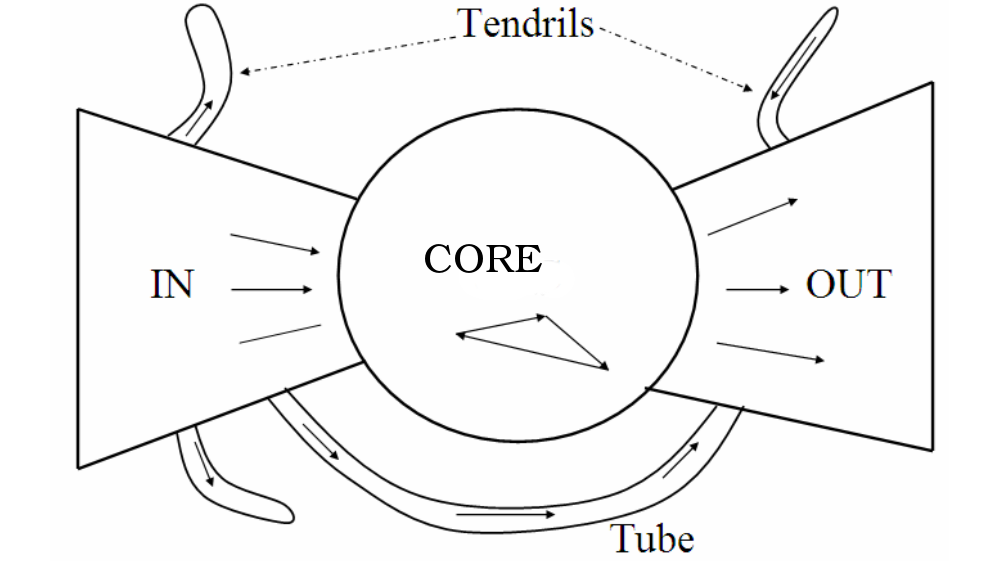
\includegraphics[height=7cm]{immagini/sub/sub}
\caption{Struttura bow-tie.}
\label{fig:sub}
\end{figure}
Il metodo elabora il grafo del web a due livelli di granularità, uno a livello di pagine web  e l'altro a livello di host. 

Il primo passo consiste nel rilevare gli host e le pagine spam partizionando il grafo in sottografi densi e calcolando delle feature per ogni sottografo sia sulla base degli URL (statistiche basate sulla lunghezza, statistiche basate sulla posizione della pagina rispetto all'homepage e statistiche basate sulla lunghezza del nome dell'host) e feature basate sul grafo. In particolare per rilevare i sottografi spam si analizza la struttura \textit{bow-tie} del grafo del web che si ottiene identificando le componenti fortemente connesse. In figura \ref{fig:sub} si nota che la struttura \textit{bow-tie} è composta da 5 elementi:
\begin{itemize}
 \item il \textit{Core} che è la componente fortemente connessa che contiene la maggior parte di siti non spam che sono facilmente accessibili agli utenti;
 \item la componente \textit{IN} è formata da pagine che puntano al \textit{Core};
 \item la componente \textit{OUT} è formata da pagine che sono puntate dal \textit{Core};
 \item le componenti \textit{Tendrils} che sono connesse alle componenti \textit{IN} o \textit{OUT} e la componente \textit{Tube}.
\end{itemize}
Quindi le pagine più facilmente accessibili sono quelle che si trovano all'interno della componente \textit{OUT}. Alcuni studi asseriscono che la presenza di dense componenti fortemente connesse vicino al \textit{Core} del grafo del web sia un indicatore potenziale di spam quindi per identificare i sottografi composti da pagine spam occorre analizzare ed individuare componenti fortemente connesse lungo \textit{In}, \textit{Out}, \textit{tendrils} e \textit{tube}.

Il secondo passo consiste nel ricondurre  a livello di host i valori di spam sia a livello di pagine che di host.

Successivamente vengono identificate le strutture fortemente connesse all'interno del \textit{Core} del grafo del web per rilevare gli host non-spam. L'identificazione dei sottografi non spam avviene all'interno della sezione \textit{Core} del grafo del web. Si definisce \textit{k-core} il massimo sottografo dove ogni nodo è connesso ad almeno \textit{k} altri nodi nel sottografo e il valore di \textit{coreness} di un nodo il massimo \textit{k} tale che il nodo venga classificato nel sottografo con il medesimo \textit{k-core}. Host molto importanti, ovvero quelli che hanno molti \textit{inlink}, sono connessi a altri host altamente connessi formando sottografi robusti con alta \textit{coreness}, mentre gli host spam hanno una bassa \textit{coreness}. Quindi impostando un certo valore di \textit{coreness} si possono identificare i sottografi con una certa robustezza e identificare soli i sottografi non spam.

Infine per aumentare il numero di host spam e non spam vengono propagati simultaneamente \textit{trustrank} e \textit{anti-trust rank}, dagli host che siamo sicuri siano non spam e spam agli host vicini in modo da valorizzare gli host non spam e penalizzare quelli di spam.

Un altro metodo per rilevare lo spam utilizza un classificatore automatico che combina un insieme di feature basate su link e contenuto \cite{Castillo:2007:KYN:1277741.1277814}. Considerando che i link tra le pagine non sono disposti in modo casuale ovvero pagine simili tendono a linkarsi tra di loro più frequentemente di pagine diverse, si può sfruttare tale meccanismo per rilevare le pagine spam che tendono a raggrupparsi in cluster. Infatti le pagine spam per aumentare il rank basato sui link utilizzano le link farm che costituiscono dei cluster all'interno del grafo. Da queste considerazioni gli autori assumono che gli host ben collegati tra di loro appartengano molto probabilmente alla stessa classe: spam o non spam.

\section{Metodi per identificare link farm}
Per riconoscere una spam farm (o link farm) si parte dal presupposto che i nodi della spam farm hanno dei link uscenti verso delle pagine target \textit{t} per aumentarne il rank. In \cite{Gyongyi:2006:LSD:1182635.1164166} per identificare le spam farm viene introdotta una misura denominata \textit{spam mass}, che valuta, basandosi sulla struttura del grafo, l'impatto dello spam sul rank di una pagina. Usando questa misura a tutte le pagine web verrano assegnati due valori: quello di \textit{pagerank} e quello relativo alla \textit{spam mass}; in particolare le pagine target delle spam farm riceveranno  un alto valore di \textit{PageRank} e un alto valore di \textit{spam mass} mentre le pagine non spam potranno  avere un alto valore di \textit{PageRank} ma un basso valore di \textit{spam mass}. Presupponendo, quindi, che il web può essere partizionato in nodi non spam \(V^+\) e nodi spam \(V^-\) e che la loro unione formi il grafo del web, per una data partizione \(\{V^+,V^-\}\) di \(V\) che contiene i nodi \(x\) il \textit{PageRank} di \(x\) è la somma dei contributi dei nodi non spam e dei nodi spam. Tenendo conto di tali presupposti, per stimare la \textit{spam mass} per ogni nodo del grafo si utilizzano due misure:
\begin{itemize}
 \item La \textit{spam mass assoluta} di \(x\), denotata con \(M_x\), è il \textit{PageRank} che \(x\) riceve dai nodi spam è che uguale a:
 \begin{equation}
   M_x=q_x^{V^-}
 \end{equation}
dove \(q_x^{V^-}\) è appunto il \textit{PageRank} di \(x\) derivato dai nodi spam.
 \item La \textit{spam mass relativa} di \(x\), denotata da \(m_x\), è la frazione del \textit{PageRank} di \(x\) dovuta al contributo dei nodi di spam cioè: 
 \begin{equation}
   m_x=q_x^{V^-}/p_x
 \end{equation}
dove \(q_x^{V^-}\) è il \textit{pagerank} di \(x\) derivato dai nodi spam e \(p_x\) il \textit{pagerank} derivato da tutti i nodi.
\end{itemize}
Dal momento che non è sempre possibile discernere la caratteristica (spam o non spam) per tutti i nodi del grafo ma solo per un sottoinsieme di nodi non spam \(\tilde{(V)}^+\) le misure precedenti vengono calcolate nel seguente modo:
\begin{itemize}
 \item la stima assoluta di \textit{spam} mass di un nodo \(x\) è:
 \begin{equation}
 \tilde{M}_x=p_x-p'_x
\end{equation}
\item la stima relativa di \textit{spam mass} di \(x\) è:
 \begin{equation}
 \tilde{m}_x=(p_x-p'_x)/p_x=1-p'_x/px
\end{equation}
\end{itemize}
dove \(p=PR(v)\) è il \textit{pagerank} dei nodi basato su una distribuzione uniforme mentre \(p'=PR(v^{\tilde{V}^+})\) è \textit{pagerank} basato sull'insieme \(\tilde{(V)}^+\)  con una distribuzione di salto \(v^{\tilde{V}^+}\). Perciò è possibile utilizzare un valore soglia tramite il quale una pagina è considerata facente parte di una spam farm se il valore della stima assoluta o relativa di \textit{spam mass} supera la soglia, perché usando \(p'\) basato sull'insieme \(\tilde{(V)}^+\) il valore di \textit{spam mass} sarà maggiore per le pagine spam. Infatti nel caso della stima assoluta di \textit{spam mass} dove \(p_x-p'_x\), \(p_x\) è maggiore rispetto a \(p'_x\) per le pagine spam in quanto avranno difficilmente una relazione con il seedset \(\tilde{(V)}^+\) e quindi la sottrazione tenderà ad avere un risultato maggiore per le pagine spam. Lo stesso ragionamento vale per la stima relativa di \textit{spam mass}.

Le pagine all'interno delle spam farm sono densamente connesse tra loro e hanno molti link in entrata e uscita. Se utilizziamo come seedset pagine note che fanno parte di una spam farm, possiamo catalogare una qualsiasi pagina come appartenente a tale spam farm se ha molti link in entrata e uscita rispettivamente da e per il seedset; in questo modo si può allargare il seedset di partenza aggiungendo la nuova pagina individuata. Tale processo è iterato fino a che nessuna altra pagina può essere aggiunta al seedset. Un metodo che applica questo principio per identificare le spam farm è descritto  in \cite{Wu05identifyinglink}. Per decidere se una pagina deve fare parte di un seedset, si parte dall'assunzione che le pagine all'interno della link farm normalmente hanno molti nodi in comune tra l'insieme dei link in entrata e quello dei link in uscita. Qualora  sono presenti pochi nodi in comune tra l'insieme dei nodi in entrata e in uscita da una pagina questa non sarà catalogata come facente parte di una link 
farm viceversa la pagina sarà catalogata facente parte della link farm. Ad esempio in figura \ref{fig:linkfarm} è rappresentata una link farm; il nodo \(A\) ha come insieme di nodi in uscita \(B\) e \(C\)  e come insieme di nodi in entrata \(B\) e \(C\), l'intersezione dei due insiemi crea un insieme di cardinalità uguale a 2, in questo caso dato le dimensioni dell'esempio il nodo \(A\) può essere considerato facente parte di una link farm.\\
Dopo avere eseguito la verifica per tutte le pagine di un dataset si può ampliare la link farm con delle nuove pagine, del grafo del web, sfruttando il fatto che se una pagina punta a un insieme di pagine spam è probabile che anche essa sia spam. Quindi se il numero di outlink di una pagina \(p\) verso la link farm è uguale o supera una soglia, la pagina sarà giudicata spam e perciò facente parte del seedset della spam farm. Una volta trovate le pagine spam bisogna utilizzare queste informazioni per il ranking. Un modo è quello di eliminare queste pagine direttamente dal grafo del web, un altro modo può essere quello di penalizzare i link invece che le pagine, facenti parte della spam farm, con un fattore di decadimento o infine potrebbe essere utile eliminare direttamente i link che fanno parte della spam farm.
\begin{figure}
\centering
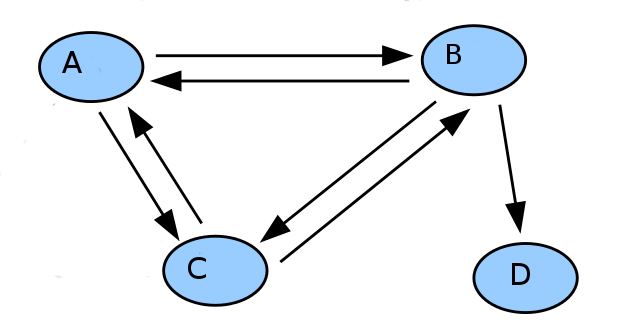
\includegraphics[width=8cm]{immagini/linkfarm/linkfarm}
\caption{Struttura di una link farm.}
\label{fig:linkfarm}
\end{figure}

\section{Link dai forum}
Un metodo utilizzato dagli spammer per creare delle grandi link farm è lo scambio di link che molto spesso avviene attraverso l'utilizzo di forum SEO (Search Engine Optimization). Questi forum contengono varie tipologie di discussioni  (ad esempio spiegazioni su come manipolare gli algoritmi dei motori di ricerca per incrementare il rank delle pagine e sezioni dedicate anche allo scambio dei link). Utilizzando tali informazioni si potrebbe costruire un algoritmo per identificare i siti spam e quindi azzerare o attenuare il loro valore di rilevanza delle ricerche in un motore di ricerca. Tale processo non è semplice in quanto la presenza di numerose e diversificate informazioni producono rumore nel rilevamento dei link. Un modo efficace per implementare questa tecnica consiste nel  \cite{Cheng:2011:LWS:1935826.1935902}: 
\begin{itemize}
 \item Estrarre tutti i link contenuti nei post.
 \item Dal momento che non tutti i link presenti nei post sono spam vengono estratte le feature dai link sulla base delle loro relazioni con gli utenti del forum e della struttura dei loro link nel grafo del web. Le feature vengono catalogate in tre tipi: feature del forum SEO (quali la frequenza di URL nel forum, il numero di thread che il proprietario dell'URL ha discusso, il numero di post autorizzati dal proprietario dell'URL, il numero di URL inseriti dal proprietario dell'URL, la media degli URL per post di un utente, il numero di post che contengono l'URL del proprietario), le feature del grafo (fra cui il numero di link in ingresso, il numero di link in uscita, la media dei link in uscita dei vicini in ingresso, la media dei link in entrata dei vicini in uscita) e le feature del sito (la lunghezza dell'URL). 
 \item Infine viene calcolato il valore di spam dei siti.
\end{itemize}
Questi metodi sono di particolare aiuto nell'incrementare il numero di pagine spam che i metodi convenzionali (sia basati sul contenuto che sulla struttura del grafo) non riescono a identificare  e perciò è possibile usarlo come metodo complementare ai metodi classici. 


\section{Metodi per migliorare la classificazione}
Oltre alla rilevazione delle pagine di spam utilizzando le tecniche e le feature descritte in precedenza, un aspetto focale consiste nel miglioramento della fase di classificazione; in \cite{Gan:2007:IWS:1244408.1244412} viene presentato un metodo per migliorare la classificazione  utilizzando un classificatore di base, per etichettare le pagine, e delle euristiche basate sulla tipologia dei nodi vicini a un nodo \(v\). Tali euristiche determinano se il nodo \(v\) dovrebbe essere rietichettato basandosi sul risultato della prima classificazione o sull'informazione tratta dalle euristiche. Gli autori di tale metodo affermano che  la struttura dei vicini di un nodo è un buon indicatore  per classificarlo in  spam o non spam. In particolare vengono analizzate alcune distribuzioni delle proprietà dei vicini:
\begin{itemize}
 \item la distribuzione dello spam in entrata: tale distribuzione è rappresentata  tramite il grafico in figura \ref{img:gan1}  dove ogni sito (di cui si conosce se esso è spam o non spam) andrà a finire in uno dei settori sull'asse \(x\) in base alla frazione di nodi spam tra i sui vicini in entrata. L'asse \(y\) rappresenta la percentuale di spam/non spam all'interno del settore. Dal grafico si nota che quanto più è alta la frazione di vicini spam in entrata di un sito tanto la probabilità che tale sito sia spam cresce.  
 \begin{figure}
 \centering
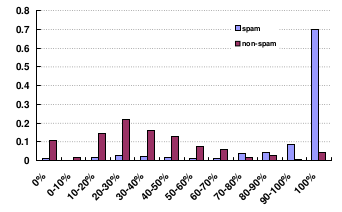
\includegraphics[width=10cm]{immagini/gan/immagine1.png}
\caption{Distribuzione dello spam in entrata}
\label{img:gan1}
\end{figure}
\item la distribuzione dello spam in uscita: tale distribuzione è rappresentata  tramite il grafico in figura \ref{img:gan2}; si osserva che tale distribuzione è simile a quella per lo spam in entrata.
 \begin{figure}
 \centering
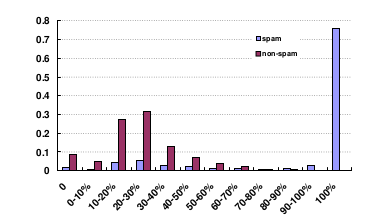
\includegraphics[width=10cm]{immagini/gan/immagine2.png}
\caption{Distribuzione dello spam in uscita}
\label{img:gan2}
\end{figure}
\item distribuzione entrante pesata: tale distribuzione è rappresentata  tramite il grafico in figura \ref{img:gan3}; in tale distribuzione vengono esaminati gli inlink pesati con pagerank.
 \begin{figure}
 \centering
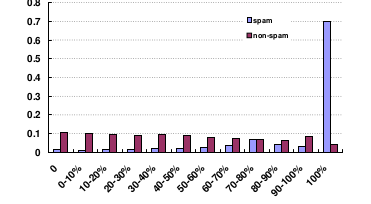
\includegraphics[width=10cm]{immagini/gan/immagine3.png}
\caption{Distribuzione entrante pesata}
\label{img:gan3}
\end{figure}
\end{itemize}
Vi sono due approcci per rietichettare i nodi dopo la prima classificazione. Nel primo, a ogni nodo viene assegnata un etichetta dal primo classificatore e successivamente viene definita un'altra etichetta per un nodo vicino, sulla base di una delle euristiche definite in precedenza, a cui viene associato un livello di confidenza; quindi l'etichetta del nodo determinata attraverso la classificazione di base viene confrontata con quella di un nodo vicino, se le due etichette sono molto difformi tra loro e l'etichetta del nodo vicino è molto affidabile in termini di confidenza allora l’etichetta del sito viene cambiata da spam a non spam (o viceversa). Il secondo modo consiste nel applicare, dopo la classificazione di base, un secondo classificatore che utilizza altre feature ( le etichette assegnate dal primo classificatore, la percentuale di inlink corrispondenti a siti spam, la percentuale di outlink che puntano a siti spam, ecc...).

Un altro metodo che fa uso della riassegnazione delle etichette associate a ogni nodo dopo una prima fase di classificazione è descritto in \cite{Geng:2008:IWS:1367497.1367685}. Tale metodo fa uso di una strategia di riestrazione delle feature facendo delle analisi basate sui clustering dei nodi, analisi sulla propagazione e analisi basate sulla struttura del grafo dei nodi vicini. L'algoritmo è suddiviso in quattro fasi:
\begin{itemize}
 \item vengono estratte delle feature base per ogni nodo;
 \item viene eseguita una prima classificazione;
 \item successivamente vengono riestratte le altre feature basate sui cluster, sulla propagazione e sulla struttura dei vicini;
 \item viene rieseguita una seconda fase di classificazione;
\end{itemize}
Le analisi sui cluster vengono eseguite utilizzando un grafo non diretto \(G=(V,E,w)\), dove \(V\) è l'insieme degli host, \(w\) è una funzione di pesatura e \(E\) è l'insieme degli archi con peso non zero. Quindi per calcolare la feature sui cluster il grafo viene partizionato in \(k\) cluster e successivamente calcolato:
\begin{equation}
 cf(H)=\frac{\sum_{h\in C(H)}spamicity(H)}{|C(H)|}
\end{equation}
dove \(C(H)\) è il cluster al quale l'host \(H\) appartiene e la \(spamicity(h)\) è il valore di spam rilevato durante la prima classificazione.\\
Diversamente la feature di propagazione si ottiene nel seguente modo:
\begin{equation}
 pf(H)^{(t)}=\sum_{h:h->H}\frac{pf(h)^{t-1}\times weight(h,H)}{\sum_{g:h->g}weight(h,g)}
\end{equation}
dove \(t\) è il numero di iterazioni, \(pf(h)^{(0)}=spamicity(h)\) e \(weigth(h,H)\) è il peso degli host \(h\) e \(H\).\\ 
Infine l'ultima feature quella relativa alla struttura dei vicini si ottiene:
\begin{equation}
 nf(H)=\frac{\sum_{h\in N(H)}(sapmicity(h)\times weight(H,h))}{|N(H)|}
\end{equation}
dove \(N(H) \in \{inlink(H), outlink(H), outlink(outlink(H)), inlink(inlink(H)),\\ inlink(outlink(H)), outlink(inlink(H))\}\) e quindi rappresenta l'insieme delle relazioni con i nodi vicini del nodo\ \(H\) .

Le prestazioni della fase di classificazione degli algoritmi di spam detection sono legate al quantità di dati di traning con cui il classificatore viene istruito.  le performance della classificazione, quindi, in \cite{Geng:2009:LBS:1526709.1526920} viene proposto un particolare algoritmo di apprendimento supervisionato denominato \textit{Link-training}; tale algoritmo si basa sull'apprendimento dai link ovvero la dipendenza topologica. L'algoritmo di apprendimento si può riassumere nei seguenti passi:
\begin{itemize}
 \item La prima fase consiste nel istruire un classificatore attraverso l'uso di un piccolo dataset.
 \item Successivamente viene utilizzato il classificatore per categorizzare e assegnare un valore di spam (\textit{PS}) ai dati non etichettati; il calcolo di \textit{PS} avviene nel seguente modo:
 \begin{equation}
  PS(x)=\frac{P_{spam}(x)}{P_{spam}(x)+P_{normal}(x)}
 \end{equation}
 dove, \(P_{spam}(x)\) è la probabilità di \(x\) di essere un nodo spam.
 \item Il passo successivo consiste nell'assegnare a tutti i nodi il valore di spam calcolato.
 \item Per istruire il classificatore oltre al valore di spam di base viene calcolato anche quello relativo ai vicini (LS):
 \begin{equation}
LS(h)=\frac{\sum_{v\in N(h)}(PS(v)\times weight(h,v))}{\sum_{v\in N(h)}weight(h,v)}
 \end{equation}
dove \(v\) e \(h\) sono gli host, \(weight(h,v)\) è il peso dell'host \(h\) e \(v\) , \(weight(h,v\in {1,\log{(n)}})\), dove \(n\) è il numero di link tra i due nodi. \(N(h)\in inlink(h) \cup outlink(h)\), dove \(inlink(h)\) rappresenta l'insieme dei link in entrata di \(h\) e \(outlink(h)\) rappresenta l'insieme dei link in uscita di \(h\). 
Queste fasi del processo sono cicliche per un numero stabilito di iterazioni.
\end{itemize}

Gli algoritmi di spam detection basati sul grafo ottenuto dalla fase di crawling sfruttano le caratteristiche dei grafi per ottenere delle informazioni riguardo i nodi spam. Quasi tutti i metodi descritti si basano sulla stessa intuizione dell'algoritmo di \textit{trustrank} (quella relativa all'isolazione approssimata delle pagine buone) sfruttando tale intuizione per determinare le pagine spam. Ad esempio \textit{Anti-trust rank} sfrutta tale intuizione ma non andando a manipolare i link in uscita di ogni nodo ma i link dei nodi entranti. Altri metodi mentre si basano sulla ricerca delle spam farm mentre altri ancora si focalizzano sul miglioramento dei vari algoritmi di classificazione. Oltre alle tecniche basate su contenuto e sul grafo del web sono state implementate altre che utilizzano criteri diversi per determinare le pagine spam che non si possono identificare tramite i metodi classici; tali metodi, quindi, sono nati per andare incontro alla crescita di nuovi tipi di web spam.





\chapter{Tecniche che fanno uso di altri segnali}
 Come già discusso nei capitoli precedenti le tecniche basate sul contenuto utilizzano delle feature determinate empiricamente su alcuni dataset di pagine web a disposizione dei ricercatori mentre le tecniche che basate sul grafo diminuiscono o eliminano del tutto l'impatto dello score dei nodi spam attraverso la determinazione di alcuni pattern strutturali all'interno del grafo.  Quindi queste nuove tecniche sono la risposta alla continua evoluzione delle tecniche di spam web. Mentre in questo capitolo saranno illustrate le tecniche di spam detection che utilizzano come segnale di partenza oggetti al di fouri del contenuto delle pagine web e della struttura del grafo. Questi nuovi tipi di approcci sono state sviluppati per identificare tutti i vari tipi di spam che hanno caratteristiche tali da non essere identificate con i metodi tradizional oppure per essere usate in modo complementare alle tecniche già presenti in letteratura ovvero quelle basate su contentuto e quelle basate sulla struttura del grafo. 


\section{Rilevamento dello spam di tipo cloacking}
Ci sono pochi metodi che tentano di rilevare il cloaking. Gli spammer possono rilevare un crawler dal suo indirizzo IP o dal campo \textit{user-agent} all'interno di una richiesta HTTP e quindi fornire due versioni di una pagina a seconda di chi effettua la richiesta. Molti dei metodi per rilevare il cloaking prendono in considerazioni due copie di una stessa pagina, la prima è ottenuta tramite un richiesta HTTP al server (che ha la pagina) da parte di un crawler e la seconda è ottenuta tramite la richiesta HTTP al server da parte del browser, quindi le due copie vengono confrontate per verificare se le due pagine siano identiche e perciò che non si tratti di cloacking. I metodi che fanno uso di questa tecnica non sono efficaci per il fatto che con l'avvento del WEB 2.0 le pagine sono generate dinamicamente e possono variare nei contenuti. Per superare l'incertezza legata alla natura dinamica delle pagine si può utilizzare un metodo \cite{Ghiam:2013cloaking} che si basa sul confronto dei termini tra le due 
copie di una pagina usando delle funzioni hash per aumentare la velocità di confronto. Il metodo definiche come  \(C_i\) l'insieme delle copie di una pagina che sono ottentute tramite le richieste fatte da parte di un crawler al server, \(B_i\) l'insieme delle copie di una pagina che sono conseguite attraverso delle richieste da parte del browser al server e s\(f\) una funzione hash allora \(f(B_i)\) e \(f(C_i)\) sono i valori di hash rispettivamente delle copie del browser e del crawler da questo ne consegue che se i valori delle due funzioni hash sono identici le pagine sono identiche in caso contrario le due pagine sono differenti. L'algoritmo contradistingue il cloacking in statico e dinamico. Nel primo caso ci si trova nella situazione in cui le copie di una pagina del browser e del crawler sono diverse mentre nel cloacking dinamico si ha esattamente la seguente situazione \(B_1=B_2=C_2 \not =C_1\) ovvero la due copie di una pagina del browser sono identiche a una copia della pagina del crawler ma sono 
differenti da un altra copia del crawler. I vari casi di cloacking statico si possono esaminare come segue:
\begin{itemize}
 \item La prima fase valuta \(f(C_1)\) e \(f(B_1)\) se i due valori di hash sono differenti vengono calcolati anche \(f(B_2)\) e \(f(C_2)\). Valori di hash differenti implicano una buona probabilità che le due pagine derivino da un meccanismo di cloacking, ma queste considerazioni non sono sufficienti perciò bisogna eseguire il passo successivo.
 
 \item In questa fase i valori di hash vengono valutati nel seguente modo: \(f(C_1)\not =f(B_1)\), \(f(C_2)\not=f(B_2)\), \(f(C_1)=f(C_2)\), \(f(B_1)=f(B_2)\). Tale valutazione suggerisce che la probabilità di cloacking è elevata ma data l'alta natura dinamica delle pagine web per essere sicuri di essere di fronte ad un meccanismo di cloacking si calcola la differenza dei termini tra \(C_1\) e \(B_1\) (denominata \(D_{C1B1}\)) che se è minore di una certa soglia allora indica che non si tratta di cloacking.
 
 \item La terza fase si contradistingue dal caso in cui \(f(C_1)\not=f(B_1)\), \(f(C_2)\not=f(B_2)\), \(f(C_1)=f(C_2)\), \(f(B_1)\not=f(B_2)\). Questo caso si differenzia dal precedente per il fato che le due copie del browser sono diverse questo suggerisce che la probabilità di cloacking è bassa e che si tratti di un contentuto altamente dinamico. Per prevenire falsi positivi vengono viene calolata \(D_1\) come le differenze dei termini tra \(C_1\) e \(B_1\) e \(D_2\) come le differenze dei termini tra \(C_2\) e \(B_2\) e succesivamente \(D_{TOTAL}\) come la differenza tra \(D_1\cup D_2\) e \(D_1 \cap D_2\). Se \(D_{TOTAL}\) è più grande di una certa soglia allora ci si trova davanti un meccanismo di cloacking.
 
 \item La quarta fase si ha con \(f(C_1)\not=f(B_1)\), \(f(C_2)\not=f(B_2)\), \(f(C_1)\not=f(C_2)\), \(f(B_1)\not=f(B_2)\), dal momento che \(f(C_1),f(C_2),f(B_1),f(B_2)\) sono differenti queste pagine cambiano molto velocemente sono pagine dinamiche. 
 
 \item Infine \(f(C_1)\not=f(B_1)\), \(f(C_2)\not=f(B_2)\), \(f(C_1)\not=f(C_2)\), \(f(B_1)=f(B_2)\), in questo caso esiste una buona probabilità di cloacking. Per determinare se la differenza tra le due copie del crawler e l'identicità tra le copie del browser indicano che si tratta di cloacking viene calcolato \(D_{C1C2}\) come la differenza dei termini tra le copie del crawler e \(D_{B1C1}\) come la differenza dei termini tra \(B_1\) e \(C1\). Se \(D_{C1C2}\) e maggiore di \(D_{B1C1}\) allora non si tratta di cloacking perchè la differenza tra le copie del crawler e maggiore della differenza tra la copia del crawler e quella del browser; questo sta a sottolineare la natura dinamica della pagina.
\end{itemize}
Per quanto riguarda il cloacking dinamico si hanno due casi: il caso in cui \(f(C_1)\not=f(B_1)\), \(f(C_2)=f(B_2)\), \(f(B_1)\not=f(B_2)\) ma non abbiamo a che fare con meccanismi di cloacking in quanto \(f(B_1)\) è diverso di \(f(B_2)\) ovvero già le due copie del browser sono diverse e quindi si tratta della pagina che cambia i contenuti a causa della sua natura dinamica ma non per fare cloacking. Mentre nel secondo caso \(f(C_1)\not=f(B_1)\), \(f(C_2)=f(B_2)\), \(f(B_1)=f(B_2)\) si nota che la copia \(C_1\) del crawler e quella \(B_1\) del browser sono diverse mentre nel secondo caso la copia del crawler \(C_2\) è uguale alla copia del browser \(B_2\). Questo significa o che il server spam sceglie quando effettuare il cloacking o che c'è una relazione con la natura dinamica delle pagine. Per questo l'algoritmo prevede il calcolo di \(D_{C1C2}\) che è uguale alla differenza dei termini tra le due copie del crawler. Se \(D_{C1C2}\) è maggiore di una certa soglia allora si tratta di cloacking.

Nella progettazione di una componente di spam detection all'interno di un crawler si protrebbe utilizzare questo metodo per rilevare il cloacking affiancandolo ad altri metodi che rilevano lo spam di altro tipo anche se questo implicherebbe che per ogni pagina ottenuta durante la fase di fetching del crawler bisognerebbe eseguire la stessa richiesta attraverso un browser. Un metodo molto più efficiente sarebbe quello di determinare il cloacking direttamente nella sola sessione del crawler.

\section{Rilevare lo spam tramite l'header HTTP}
Un metodo innovativo per rilevare lo spam è quello descritto in \cite{Webb:2008:PWS:1458082.1458129}. Tale metodo può essere usato come supporto ad altri metodi descritti in precedenza e può essere utilizzato in modo dinamico durante la fase di downloading delle pagine, utile per risparmiare il numero di richieste inutili verso pagine spam. Diversamente dai metodi classici (basati sull'uso del contenuto della pagina o sulla struttura del grafo) questo metodo utilizza le informazioni racchiuse all'interno dell'header HTTP per determinare le pagine spam. Oltre all'utilizzo lato server (crawler) può essere usato anche lato client per migliorare la qualità dei contenuti protegendo da malware e permettendo di riparmiare banda e quantità di memoria. Infatti prima viene effetuata una richiesta HTTP, al server, per una pagina ma durante la lettura della pagina ci si ferma al solo header; successivamente viene azionato un classificatore per valuare l'header come spam o non spam; se l'header viene classificato come 
non spam allora si continua con la lettura del resto della pagina. I vari campi all'interno delle sessioni HTTP possono essere usate come feature che sono poi valutate dal classificatore. Analizzando i vari campi si nota che le pagine spam hanno molto frequentemente alcuni campi rispetto alle pagine non spam che hanno gli stessi campi con minore probabilità. Ad esempio in figura \ref{img:webb1} vengono confrontate le distribuzioni degli indirizzi IP per il corpus di pagine WebSpam (che contiene delle pagine spam) e il corpus WebBase (che contiene pagine non spam); dal grafico si nota che gli indirizzi IP nel corpus WebSpam sono concentrati principalmente nel range tra \(63.* - 69.*\) e \(204.* - 216.*\).
\begin{figure}
\centering
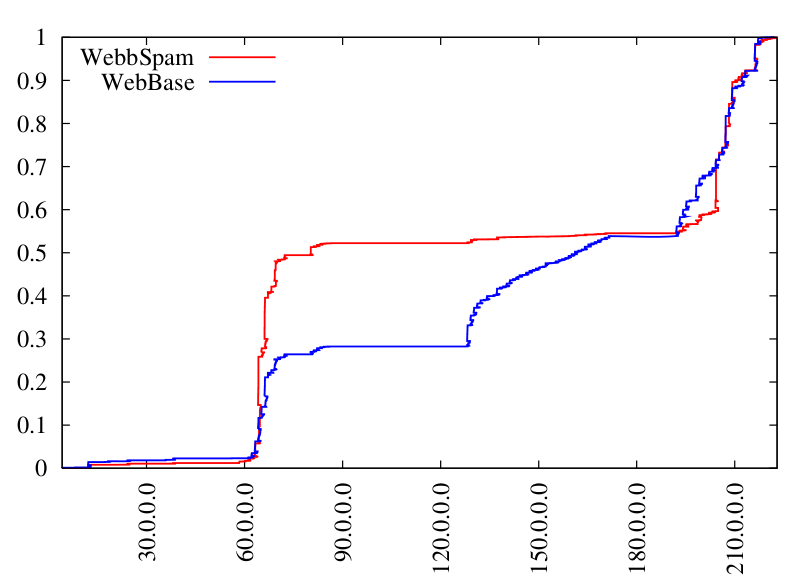
\includegraphics[width=10cm]{immagini/altre/webb.png}
\caption{Distribuzione degli indirizzi IP di due dataset: WebSpam che contiene pagine spam e WebBase che contiene pagine non spam.}
\label{img:webb1}
\end{figure}
Perciò tale metodo tenta di fare uso dell'header HTTP in modo tale da classificare le pagine basandosi sull'osservazione che pagine spam e pagine non spam	 hanno valori (campi dell'header) che hanno distribuzioni distinte. Questo metodo comunque non è molto affidabile se usato da solo perciò è un ottimo strumento da usare in modo complementare ad altri metodi più tradizionali. Un uso sensato sarebbe quello di utilizzare questa tecnica come processo di preselezione in modo tale da sfoltire il numero di pagine che gli altri metodi (che si basano o sull'uso del contenuto delle pagine o del grafo del web) devono utilizzare e quindi richiedendo un numero minore di risorse.

\section{Altri metodi}
 Nuovi metodi di spam detection fanno uso di pattern basati sul comportamento dell'utente per identificare le pagine spam come in \cite{Liu:2008:UBO:1367497.1367645}  un metodo che identifica le pagine spam che fa uso di tre feature ricavate da pattern comportamentali basati sulle azioni dell'utente in presenza di  pagine spam e pagine non spam. Le feature sono cosi calcolate:
\begin{itemize}
 \item La prima feature è denominata SEOV (Search Engine Oriented Visit) ed è definita come:
 \begin{equation}
  SEOV(p)=\frac{\#(Search\ engine\ oriented\ visit\ of\ p)}{\#(Visit\ of\ p)}
 \end{equation}
  dove \(p\) rappresenta la pagina web per cui viene calcolata la feature. La misura al numeratore indica la visita della pagina \(p\) per mezzo dei motori di ricerca mentre la misura denominatore indica la visita alla pagina \(p\) senza il bisogno di utilizzare i motori di ricerca. Dato che un utente non andrebbe mai su pagine spam se non ingannato dai risultati dei motori di ricerca, le pagine spam hanno valori alti per questa feature. In figura \ref{img:seov} è rappresenta la distribuzione delle pagine (del dataset usato dagli autori) sulla base del valore della feature SEOV; in rosso sono rappresentate le pagine spam mentre in blu sono rappresentate le pagine non spam. Molte pagine web spam hanno valori SEOV più alti delle pagine non spam perchè i motori di ricerca sono gli strumenti, e in alcuni casi sono gli unici, tramite cui le pagine spam possono essere raggiunte.
\begin{figure}
\centering
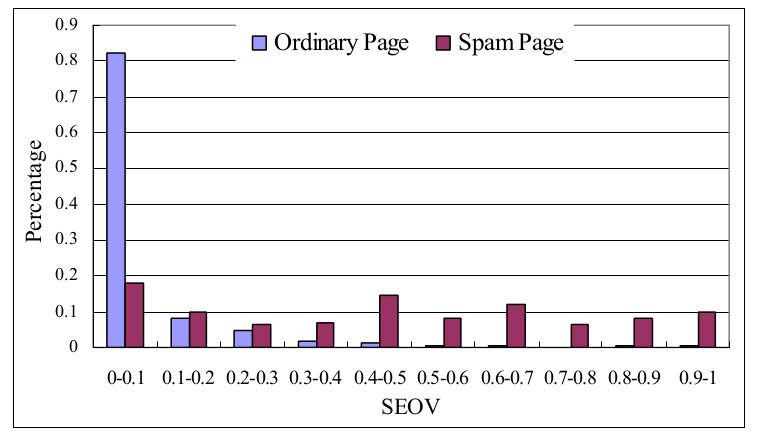
\includegraphics[width=10cm]{immagini/altre/seov.png}
\caption{Distribuizione delle pagine sulla base della feature SEOV.}
\label{img:seov}
\end{figure}
  
 \item Visto che esiste una grande differenza tra chi progetta una pagina spam e chi ne progetta una non spam, ci si avvale del comportamento dell'utente per etichettare le pagine. Un utente rimane su una pagina spam solo fino a al punto in cui capisce di essere su un sito con contenuti non pertinenti, mentre nel caso in cui si trovi a navigare su una pagina non spam l'utente è stimolato a rimanrci. Quindi la seconda feature è definita come SP (Start Point Visiting rate):
 \begin{equation}
  SP(p)=\frac{\#(user\ click\ a\ hyperlink\ on\ p\ while\ visiting\ p)}{\#(Visit\ of\ p)}
 \end{equation}
 questa feature indica quanti click sono fatti su una certa pagina \(p\).
 \item Infine l'ultima feature è denominata SN (Short-term Navigation rate) e indica quante pagine di un sito \(w\) saranno visitate una volta che un utente visita il sito \(w\). Questa misura è definita in questo modo:
 \begin{equation}
  SN(w)=\frac{\#(Session\ in\ wich\ users\ visit\ less\ than\ N\ pages\ in\ w)}{\#(Session\ in\ wich\ user\ visit\ w)}
 \end{equation}
 \end{itemize}
Qundi questo metodo utilizzando pattern comportamentali per determinare le pagine spam è molto più flessibile dei metodi tradizionali, i quali sono dipendenti dalla struttura della pagina o del grafo. La novità di questo metodo sta nel fatto che mentre gli altri metodi sono basati sullo studio di determinate proprietà che le pagine web hanno (nel caso dei metodi basati sul contenuto delle pagine) o sullo studio del grafo del web e la tipologia che le pagine web assumo all'interno quest'ultimo metodo si basa sul comportamento dell'utente. Questo rende il problema dell'identificazione dello spam scalabile ovvero protrebbe riuscire ad arginare e rilevare anche le nuove tipologie di spam web che potrebbero essere implementate mentre con i metodi classici è più difficile in quanto si basano su delle euristiche riscontrate su alcuni dataset e quindi sono dipendenti dalla tipologia di spam che si riscontra e non sono mutabili ovvero non possono essere flessibili per apprendere i nuovi tipi di tecniche spam.

Ci sono altri metodi che fanno uso del comportamento dell'utente durante la navigazione web per determinare le pagine spam molto innovativo e interessante è \textit{BrowseRank} \cite{Liu:2008:BLW:1390334.1390412}. \textit{BrowseRank} determina l'importanza di una pagina web dal grafo ricavato dal comportamento dell'utente durante la navigazione web con il browser. Il grafo è costituito dai vertici che rappresentano le pagine. da archi orientati che rappresentano le transizioni da una pagina all'altra da parte dell'utente e anche dal tempo di permanenza su una pagina. Infine come per \textit{Pagerank} viene utilizzato il grafo ricavato per determinare l'importanza delle pagine. In figura \ref{img:browser} è rappresentato uno schema esplicativo del modo con cui si ricava il grafo. Il grafo è ricavato dai browser degli utenti (ad esempio tramite l'utlizzo di toolbar) che raccolgono diversi dati come l'URL, il tempo di permanenza, la tipologia della visita (ad esempio se l'utente ha inserito l'URL nella barra 
degli indirizzi del browser oppure se arrivato a ad una pagina per mezzo di un link) e vegono poi recuperati da un server che integra i dati provenienti da milioni di utenti.
\begin{figure}
\centering
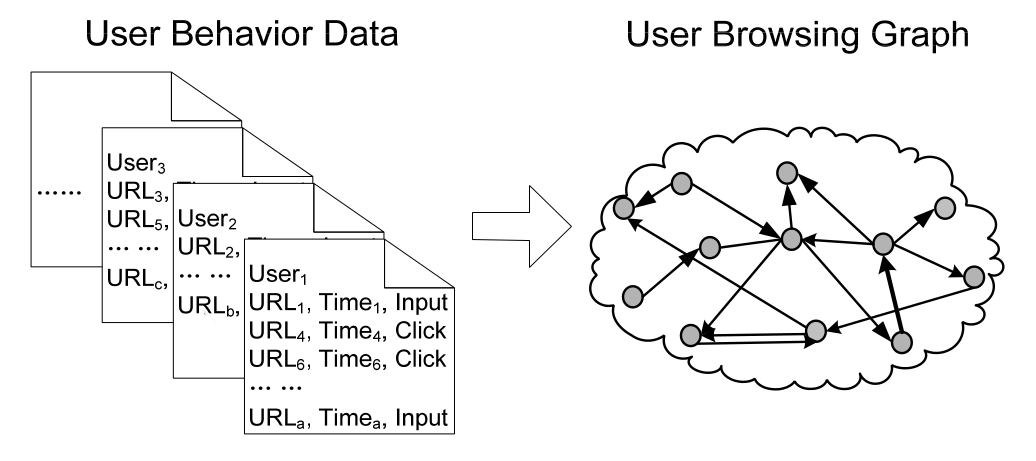
\includegraphics[width=10cm]{immagini/altre/browser.png}
\caption{Dal comportamento dell'utente al grafo.}
\label{img:browser}
\end{figure}
Questo algoritmo ha due vantaggi principali rispetto ai metodi tradizionali sui link quali:
\begin{itemize}
 \item Dato che il grafo è ricavato durante la fase di navigazione è più accurato di quello ricavato da un crawler perché i link tra le pagine possono cambiare continuamente.
 \item Questo metodo inoltre tiene conto anche del tempo in cui ci si sofferma su una pagina, caratteristica che può fare capire se si è in presenza di una pagina spam, infatti un utente non avrebbe nessun vantaggio a rimanere a lungo su una pagina con poca pertinezza e qualità rispetto al suo bisogna di informazione.
\end{itemize}
Dagli esperimenti gli autori hanno notato che \textit{BrowseRank} è più efficiente rispetto a \textit{Trustrank} e quindi dimostra che i metodi che si basano su segnali differenti dal contenuto o dal grafo del web possono essere in grado di lavorare autonomamente e non solo in modo  complementare ai metodi classici.

Un ultimo metodo \cite{Wei:2012:FAW:2348283.2348338} per rilevare lo spam web affronta  il problema da un altro punto di vista: gli autori hanno osservato che le query più comuni (quelle che hanno un alta frequenza nei file log dei motori di ricerca) sono  quelle che genereranno più spam. Tali query hanno le seguenti caratteristiche: sono molto comuni e quindi riflettono una grande quantità di richiesta da parte degli utenti, e i risultati per queste query sono composti da pochi risultati utili in quanto sono prese di mira per fare spam ovvero le pagine spam molte volte sono piene di pubblicità e per attirare l'utente (o meglio per ingannarlo) cercano di manipolare i motori di ricerca per andare in cima ai risultati quindi le query più popolari saranno prese di mira più frequentemnte da chi fa spam. Il metodo, tenendo conto di queste considerazioni, fa uso dei file log dei click dei motori di ricerca per prevenire lo spam web.

\chapter{Dataset e strumenti utilizzati}
\lstset{basicstyle=\small\ttfamily,keywordstyle=\color{black}\bfseries,commentstyle=\color{darkgray},stringstyle=\color{black},showstringspaces=true} 
Questo capitolo illustra il dataset utilizzato per l'implementazione e l'esecuzione dei test,  discussi nel capitolo successivo, e gli strumenti (tra cui framework e librerie) utilizzate per rendere più efficienti i vari test.
\section{Descrizione del dataset}
Il dataset utilizzato per gli espirementi è WEBSPAM-UK2007 \cite{webspam-uk2007} ottenuto da un crawl del dominio ``.uk'' nel maggio del 2007 tramite il supporto del ``Laboratorio di Algoritmica per il Web'' dell'Università degli Studi di Milano; è composto da un insieme di 105.896.555 pagine che fanno parte di 114.529 host. Gli host del dataset, per mezzo del supporto  di alcuni volontari,  sono stati etichiettati in due classi: nodi spam e nodi non spam . Il dataset è composto da tre parti:
\begin{itemize}
 \item La prima parte contien le etichette associate agli host (divise in due gruppi). Il primo gruppo è costituito da 2/3 dell'insieme degli host valutati, ed è pensato stato pensato per essere utilizzato come dataset di traning. Questo primo gruppo è costituito da 3776 nodi etichettati come non spam, 222 nodi etichettati spam ed infine 277 nodi etichettati ``undecided'' ovvero nodi di cui la natura (spam o non spam) è in dubbio. Il secondo gruppo di etichette costituito dal rimanente 1/3 dell'insieme degli host valutati, è stato pensato per essere utilizzato come dataset di testing. Il secondo gruopo è costituito da 1933 nodi etichettati non spam, 122 nodi etichettati spam e 149 etichettati ``undecided''.\\
 L'assegnazione di un'etichetta ad un host avviene in due fasi. Nella prima fase l'utente valutatore ha a disposizione il contenuto della collezione e la lista degli host collegati per ogni host valutato. Nella seconda fase, invece, all'utente valutatore vengono fornite l'etichette  assegnate da altri utenti ad un host e gli viene chiesto di rivalutare le sue valutazioni se è in disaccordo con altri. Quindi viene realizzato un file che contiene tali informazioni.\\ 
 Gli host sono identificati attraverso un \textit{id} che va da 0 a 114.528 a cui è associato l'URL corrispondente. Quindi un file specifica, per ogni host valutato, il suo \textit{id}  e l'etichetta associata tra ``nonspam'',``spam'' e ``undecided'', oltre all'etichetta vengono associate le singole valutazioni effettuate dagli utenti e la media risultante delle valutazioni effettuate per quell'host tenendo conto che l'etichetta spam è uguale a 1, l'etichetta non spam è uguale a 0 e l'etichetta di ``undecided'' ha valore 0.5. Un esempio è rappresentato di seguito: 
 \begin{lstlisting}[frame=trbl,postbreak=\space, breakindent=5pt, breaklines]
ID ETICHETTA MEDIA VALUTAZIONI
5 nonspam 0.00000 j1:N,j2:N
100 nonspam 0.33333 j14:N,j17:S,j7:N
120 spam 1.00000 j18:U,j4:S
170 undecided - j13:U,j20:U
210 undecided 0.50000 j15:N,j16:S,j22:U
\end{lstlisting}
Nell'esempio vengono rappresentati 5 host; prendendo in cosiderazione l'host con \textit{id} uguale a 5 si nota subito che è stato giudicato come nodo non spam e che la media delle due votazioni è uguale a 0 visto che entrambi gli utenti hanno giudicato il nodo non spam (es. j1:N; \(N\) indica non spam, \(S\) indica spam e \(U\) indica che la natura del nodo non è definita).\\ 
Comunque per i test da eseguire tutte queste informazioni sono superflue, e dal momento che avevamo solo il bisogno di sapere quali nodi fossero spam e quali non spam sono stati utilizzati solo i dati relativi alle etichette associate ai nodi del primo gruppo.

 
 \item La seconda parte contiene il grafo definito con due differenti livelli di granularità. Quindi ci sono due grafi uno definito a livello di host mentre un secondo grafo è definito a livello di pagina. Il grafo a livello di host (che poi sarà quello utilizzato per eseguire i test) è formato da 114.528 nodi (rappresentanti gli host) mentre il secondo è formato  105.896.555 di nodi (rappresentanti le pagine web)  connessi da circa 3.7 miliardi di archi (ovvero i link tra le pagine). Il grafo degli host gestisce i link mutipli tra gli URL aggregando i vari link tra le pagine di differenti host in un singolo link a cui è associato un peso.\\
 Il file che descrive il grafo a livello di host ha una particolare sintassi: la prima riga indica il numero di host nel grafo mentre le successive righe contengono gli \textit{outlink} degli host, ad esempio alla riga due verranno indicati gli \textit{outlink} del nodo 0 alla riga tre gli \textit{outlink} del nodo 1 e cosi via. Dato che i link sono pesati la sintassi completa per ogni riga che rappressenta un nodo è:
 $$
 dest_1:nlinks_1,dest_2:nlinks_2,...,dest_k:nlinks_k
 $$
 dove \(dest\) è il nodo di arrivo del link ed è rappresentato dall'\textit{id} del nodo di destinazione mentre \(nlinks\) è il numero di link tra le pagine dei due host.
 Ad esempio di seguito è illustrato una porzione di un grafo degli host:
\begin{lstlisting}[frame=trbl,postbreak=\space, breakindent=5pt, breaklines]
114529
1005:1 8306:1 9596:1 
8107:3320 22950:4 108053:1
24003:1
24003:1
...
\end{lstlisting}
Nella prima riga dell'esempio viene specificato che il grafo è composto da 114529 nodi. Nella seconda riga si nota che il nodo 0 ha 3 outlink, uno verso il nodo 1005, un altro link verso il nodo 9596 ed infine un link verso il nodo 8306. La terza riga indica che il nodo 1 ha 3 outlink: un link verso il nodo 8107 con un peso 3320 (quindi le pagine del nodo 1 hanno 3320 link verso le pagine del nodo 8107), un link verso il nodo 22950 con peso 4 ed infine un link verso il nodo 108053. Il file quindi sarà lungo 114530 righe.\\
%nel nostro caso non sono state usate le informazioni sui pesi degli archi si è scelto di eliminare tale informazione
Quindi utilizzando queste informazioni si può convertire il file che descrive il grafo in  in modo da poter essere successivamente manipolato tramite il framework WebGraph \cite{Boldi03thewebgraph}.
%si può inserire come fare la conversione
\item La terza parte contiene il contenuto delle pagine HTML fornito in formato WARC. ``Il formato WARC specifica un metodo per combinare molte risorse in un unico file con le relative informazioni'' (\url{http://www.digitalpreservation.gov/formats/fdd/fdd000236.shtml} il 5/5/2014).
\end{itemize}

Quindi per lo sviluppo dei test sono state utilizzate due informazioni utili derivate dal dataset: le etichette che identificano i nodi del grafo spam da quelli che sono non spam e la struttura del grafo che verrà manipolata tramite l'utilizzo del framework WebGraph \cite{Boldi03thewebgraph}. WebGraph è un framework per la compressione di enormi grafi e permette, quindi, di eseguire operazioni sul grafo in maniera molto semplice e veloce. 

\section{La Tau di Kendall}
Alcuni test che sono stati implementati hanno come obbiettivo il calcolo della distanza tra due vettori e quindi per tale motivo è stata utilizzata la Tau di Kendall \cite{KendallTau}. Più precisamente la Tau di Kendall valuta il grado di similarità tra due vettori ovvero dati due vettori \(r_i\) e \(s_i\) con \(i=0,1,...,n-1\) e \(i<j\), si dice che una coppia \((i,j)\) è:
\begin{itemize}
 \item \textit{concordante} se \(r_i-r_j\) e \(s_i-s_j\) sono entrambe diverse da 0 e hanno lo stesso segno;
 \item \textit{discordante} se \(r_i-r_j\) e \(s_i-s_j\) sono entrambe diverse da 0 e hanno segno opposto;
 \item \textit{r-tie} se \(r_i-r_j=0\);
 \item \textit{s-tie} se \(s_i-s_j=0\);
 \item \textit{joint tie} se \(r_i-r_j=0\) e \(s_i-s_j=0\).
\end{itemize}
Allora viene definito  \(C\) come il numero delle coppie concordanti, \(D\) il numero delle coppie discordanti, \(T_r\) il numero delle coppie r-tie, \(T_s\) il numero delle coppie s-tie ,\(J\) il numero delle coppie joint tie e \(N=n(n-1)/2\). Quindi \(C+D+T_r+T_s-J = N\). La Tau di Kendall può essere calcolata come:
\begin{equation}
 \tau = \frac{(C-D)}{[(N-T_r)(N-T_S)]^{1/2}}
\end{equation}
Per eseguire i test è stato scelto di usare la libreria  ``it.unimi.dsi.law'' \cite{libreriaLaw} fornita dal LAW (Laboratori di Algoritmica per il Web) dell'Università degli studi di Milano. Questa libreria contiene dei metodi che consentono di calcolare efficientemente la Tau di Kendall.

\section{Il framework Webgraph}
Per la gestione del grafo è stato usato il framework WebGraph \cite{Boldi03thewebgraph}. Questo framework permette di comprimere i grafi e di eseguire delle operazioni su di essi in maniera molto efficiente. Nell'implementazione dei test viene utilizzata solo una piccola parte delle risorse che mette a disposizine WebGraph. Infatti esso incorpora:
\begin{itemize}
 \item un insieme di codici di compressione per la memorizzazione dei grafi;
 \item algoritmi che permettono di accedere al grafo compresso senza ogni volta doverlo decomprimere;
 \item algoritmi di analisi dei grafi;
 \item insiemi di dati che si possono analizzare.
\end{itemize}
Dal momento che i nostri test esaminano delle proprietà di alcuni algoritmi sui grafi, questo framework rende le operazioni molto efficienti.


\chapter{Test dei metodi di spam detection}
\lstset{basicstyle=\small\ttfamily,keywordstyle=\color{black}\bfseries,commentstyle=\color{darkgray},stringstyle=\color{black},showstringspaces=true} 
Nei capitoli precendenti sono stati illustrati vari metodi che di spam detection classificati basandosi sui segnali in ingresso che essi hanno bisogno per poter identificare le pagine web; quindi si hanno tre classi: metodi basati sul contenuto, metodi basati sul grafo e metodi che utilizzano segnali diversi dai primi due. Tra questi metodi ne sono stati presi in esame due: \textit{Trustrank} e \textit{Anti-trust rank}. 

Si è scelto, quindi, di valutare l'efficacia di due  algoritmi \textit{linked base} (\textit{Trustrank} e \textit{Anti-trust rank}) se essi operassero in modo online. Più precisamente i vari test consistono nel verificare quanto questi due algoritmi di tipo offline riescano ad approssimare il loro comportamento se li facessimo operare in modo online ovvero durante la fase di crawling. Le domande che ci poniamo eseguendo questi test su i due algoritmi di spam dection offline (\textit{Trustrank} e \textit{Anti-trus rank}) sono:
\begin{itemize}
 \item possono questi algoritmi essere in grado di operare in modalità online?
 \item durante l'esecuzione in modalità online, quanto riescono ad approssimare il loro comportamento offline?
 \item è conveniente utilizzare questi algoritmi in modalità online?
\end{itemize}

E' doveroso specificare che un algoritmo di spam detection lavora offline se questo viene eseguito dopo l'attività di crawling (e quindi dopo che si ha a disposizione l'intero grafo ottenuto dai collegamenti tra le pagine), mentre un algoritmo di spam detection lavora online se questo viene eseguito durante il processo di crawling e quindi riesce a determinare all'istante se una pagina deve essere considerata spam o non spam. Dal momento che si è scelto di esaminare degli algoritmi \textit{linked base}, e sapendo che questi formulano delle conclusioni sulla natura delle pagine (ovvero se sono spam o non spam) esaminando la struttura dell'intero grafo, è interessante notare come questi si comportino se il grafo su cui fare le valutazioni è incompleto.
%altre considerazioni

Il capitolo è diviso nel seguente modo: nella prima parte verrà illustrato come è stato scelto di simulare il crawler per poter eseguire gli algoritmi offline duratne la fase di crawling; nella seconda parte verrà spiegato come sono stati implementati i test; infine verrano illustrati tutti i test.

\section{Simulazione del crawler}
Per simulare il comportamento di crawler, e quindi eseguire gli algoritmi di \textit{Trustrank} e \textit{Anti-trust rank}, abbiamo implementato una semplice visita sul grafo in ampiezza ovvero una BFS \cite{bfsCormen} (Breadth-First Search). La visita in ampiezza dato un grafo \(G=(V,E)\), dove \(V\) è l'insieme dei vertici del grafo ed \(E\) l'insieme degli archi del grafo, e un vertice \(s\) da cui far partire la visita, scopre tutti i vertici che sono raggiungibili da \(s\). La visita in ampiezza scopre tutti i vertici che si trovano a distanza \(f\) dal vertice di partenza e successivamente scopre i vertici che si trovano a una distanza successiva \(f+1\). In sostanza dato il nodo di partenza \(s\), la visita in ampiezza, scopre tutti i nodi vicini al nodo \(s\) e successivamente per ogni nodo vicino scoperto trova i vicini che non sono ancora stati visitati; questo processo viene iterato finche tutti i nodi del grafo raggiungibili da \(s\) sono visitati. \\
Quindi anziche implementarci l'algoritmo BFS abbiamo utilizzato l'implementazione definita nel framework WebGraph. In particolare è stata utilizzata la classe ``ParallelBreadthFirstVisit'' che esegue una visita in ampiezza utilizzando il parallelismo derivato dai processori multicore.

\section{I test}
Come gia introdotto lo scopo dei test consiste che dato un algoritmo di spam detection che opera in modo offline valutare le sue prestazioni se operasse in modo online. Oltre tutto abbiamo scelto due algoritmi \textit{linked base} quali \textit{Trustrank} e \textit{Anti-trust rank} questo significa che l'algoritmo opererà su un grafo del web incompleto, all'inizio del crawling, fino ad arrivare ad operare sull'intero grafo alla fine del crawling.

\begin{figure}
\centering
 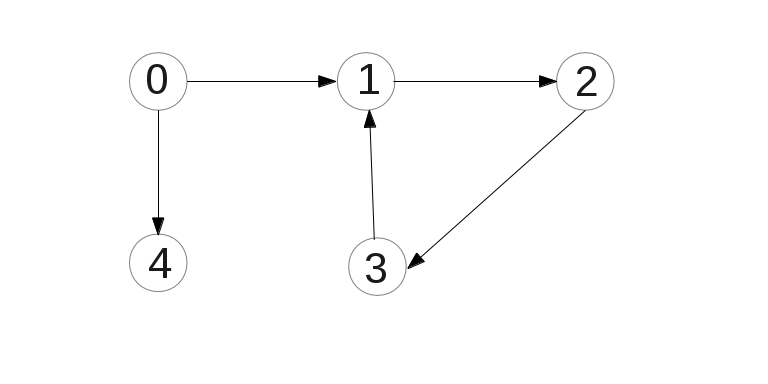
\includegraphics{immagini/test/grafoComp}
 \caption{Esempio di grafo}
 \label{fig:grafoComp}
\end{figure}

Quasi tutti i test seguono uno stesso schema; viene eseguito \textit{Trustrank} (e \textit{Anti-trust rank}) sul grafo completo, e lo indicheremo con \(t\) (\textit{Anti-trust rank} sarà indicato con \(a\)), successivamente viene eseguita la BFS (ovvero la visita in ampiezza) con nodo sorgente \(s\) e quindi si ricava la coda \(q\) dei nodi visitati a partire da \(s\); dopo di che si calcola \textit{Trustrank} (e \textit{Anti-trust rank}) sul grafo ricavati lungo la visita in ampiezza formato, quindi, da un sottoinsieme di nodi \(q\), il risultato lo indicheremo con \(\hat{t}_i\) (\textit{Anti-trust rank} sarà indicato con \(\hat{a}_i\)) dove \(i\) è il numero di nodi presi in considerazione dalla coda \(q\). Questo processo viene iterato incrementando sempre di più l'intervallo \(i\) finché non si arriva alla fine della coda \(q\) dei nodi visitati partendo dal nodo \(s\). Dopo aver calcolato \(t\) e \(\hat{t}_i\) sono due vettori si possono valutare tramite la Tau di Kendall e indicheremo con \(\tau(t,\hat{
t}_i)\) la Tau di Kendall per \(t\) e \(\hat{t}_i\)  (e quindi \(\tau(a,\hat{a}_i)\) sarà la Tau di Kendall per \(a\) e \(\hat{a}_i\)). Ad esempio in figura \ref{fig:grafoComp} è rappresentato il grafo completo su cui verra calolato \(t\) e \(a\) mentre in figura \ref{fig:grafo3} è rappresentato il grafo ricavato dalla BFS eseguita sul grafo precedente partendo dal nodo 1; se si considerano tutti i nodi lungo la visita il vettore di \textit{trustrank} sarà \(\hat{t}_3\) mentre quello di \textit{anti-trust rank} sara \(\hat{a}_3\)..

 \begin{figure}
\centering
 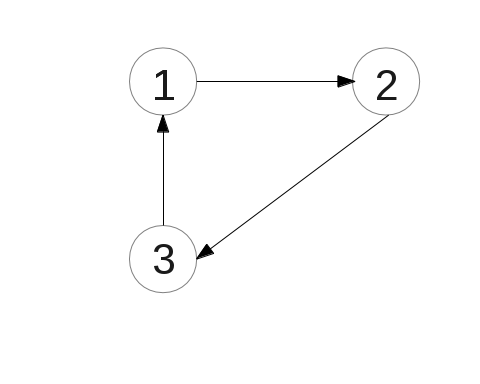
\includegraphics{immagini/test/grafo3}
 \caption{Esempio di grafo ricavato tramite una BFS a partire dal nodo 1 del grafo in figura \ref{fig:grafoComp}.}
 \label{fig:grafo3}
\end{figure}
A ogni indice del  vettore di \textit{Trustrank} \(t\) e del vettore di \textit{Anti-trust rank} \(a\) corrisponderà un nodo è il valore del vettore per un dato indice indica il valore di \textit{Trustrank} e \textit{Anti-trust rank} del nodo del grafo. In figura \ref{fig:tVettore} è illustrato un esempio del vettore di \textit{trustrank} calcolato sull'intero grafo e in figura \ref{fig:aVettore} è illustrato un esempio del vettore di \textit{anti-trust rank} calcolato sull'intero grafo. 
Nell'esempio in figura \ref{fig:tVettore} si nota che il vettore \(t\) di \textit{trustrank} ha lunghezza 5, quindi il grafo sarà composto da 5 nodi dove ad ogni nodo è associato il valore di \textit{trustrank}. Le stesse considerazioni valgono per l'esempio in figura \ref{fig:aVettore} dove il vettore di \textit{anti-trust rank} è ha lunghezza 5 e quindi l'algoritmo opererà su un grafo composto da 5 nodi.

\begin{figure}
\centering
 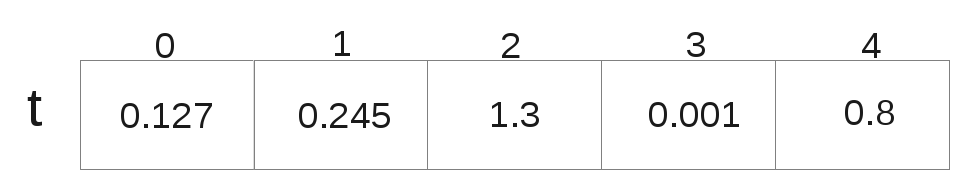
\includegraphics{immagini/test/trustVettore}
 \caption{Esempio del vettore di trustrank calcolato sull'intero grafo}
 \label{fig:tVettore}
\end{figure}
\begin{figure}
\centering
 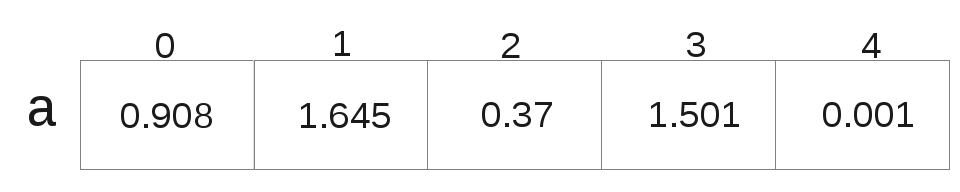
\includegraphics{immagini/test/immagineAntiTrust}
 \caption{Esempio del vettore di anti-trust rank calcolato sull'intero grafo}
 \label{fig:aVettore}
\end{figure}

A differenza dei vettori \(t\) e \(a\) (\textit{trustrank} eseguito sull'intero grafo e \textit{anti-trust rank} sull'intero grafo) , dove ad ogni indice (cioè ad ogni nodo) è associato un valore di \textit{trustrank} e \textit{anti-trust rank} , i vettori \(\hat{t}_i\) e \(\hat{a}_i\) non avranno per ogni indice un valore associato. Più precisamente, sapendo che \(\hat{t}_i\) e \(\hat{a}_i\) sono calcolati durante l'esecuzione di una BFS allora a ogni passo ci saranno ancora dei nodi da visitare per cui non è possibile calcolare i valori di \textit{trustrank} e \textit{anti-trust rank}, perciò con l'avanzamento della visita in ampieza sempre più nodi avranno associato un valore di \textit{trustrank} e \textit{anti-trust rank}. Vale quindi che \(\hat{t}_{i+1}\) avrà molti più nodi per cui è stato calcolato \textit{trustrank} rispetto a \(\hat{t}_i\) (lo stesso comportamento si riscontra per \textit{anti-trust rank}). Inoltre non è detto che dopo aver terminato la visita in ampiezza, partendo da un nodo \(s\),
 si sia visitato tutto il grafo (ovvero che \(s\) può raggiungere tutti i nodi del grafo) perciò in questo caso \(\hat{t}_i\) e \(\hat{a}_i\) avranno un numero minore di nodi per cui è calcolato \textit{trustrank} e \textit{anti-trust rank} rispetto a \(t\) e \(a\).\\
Dal momento che la Tau di Kendall tra due vettori, per essere eseguita, richiede che i due vettori abbiano la stessa lunghezza allora bisogna gestire i casi in cui i nodi del grafo temporaneo (ottenuto ad ogni intervallo di nodi visitato tramite la visita in ampiezza) non abbiano associato un valore. Per gestire tale problema si è scelto di considereare i soli nodi compresi nel grafo temporaneo. Ad esempio in figura \ref{fig:tBFSmodoB} viene illustrato il caso in cui eseguendo la BFS dal nodo 1, i nodi 0 e 4 rimangano senza aver assegnato un valore di \textit{trustrank}. Quindi gli indici 0 e 4 del vettore \(t\) non sono inclusi nel vettore \(\hat{t}_3\) questo implica che ci deve essere una corrispondenza tra gli indice del vettore \(t\) e quelli del vettore \(\hat{t}_3\) (in figura \ref{fig:tBFSmodoB} l'indice 0 del vettore \(\hat{t}_3\) corrisponde all'indice 1 del vettore \(t\), l'indice 1 al indice 2 ed infine l'indice 2 all'indice 3).  Si inoltre nota che il vettore \(\hat{t}_3\) ha lunghezza inferiore 
al vettore \(t\). Inoltre il calcolo della Tau di Kendall sara tra il vettore \(t\) formato dai soli indici compresi nel vettore \(\hat{t}_i\) e dal vettore \(\hat{t}_i\). Quindi  nella valutazione  il vettore \(t\) dovra essere ristretto alla lunghezza del vettore \(\hat{t}_i\) e quindi dovranno essere eliminati gli indici del vettore \(t\) che non sono inclusi nel vettore \(\hat{t}_i\).
\begin{figure}
\centering
 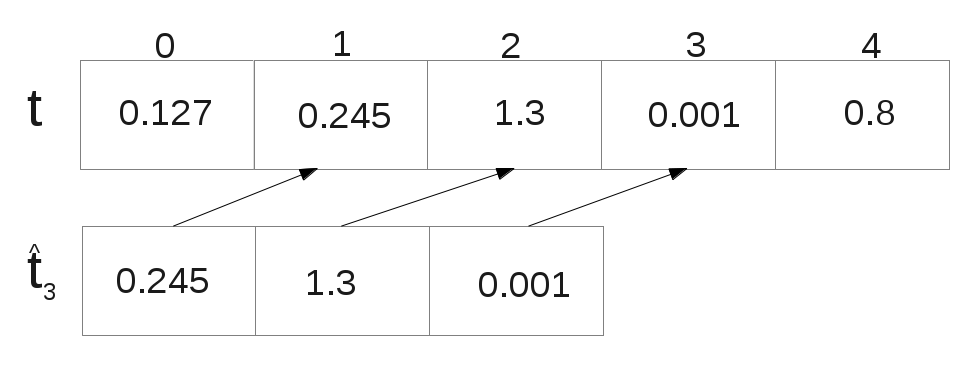
\includegraphics{immagini/test/tBFSmodoB}
 \caption{Esempio del vettore di trustrank calcolato su una porzione di grafo.}
 \label{fig:tBFSmodoB}
\end{figure}
Un altro metodo che può essere utilizzato è quello di assegnare ad ogni indice dei vettori \(\hat{t}_i\) e \(\hat{a}_i\) non ancora visitati il valore 0.0. Ad esempio prendendo in considerazione il grafo in figura \ref{fig:grafoComp} e ipotizzando di eseguire una BFS a partire dal nodo 1 e di aver visitato i nodi 2 e 3 quindi se calcoliamo \textit{trustrank} e \textit{anti-trust rank} sul sottografo ricavato dai nodi visitati, i nodi 0 e 4 avranno associato i valori 0.0 (usando il metodo \textit{Modo\_A}), tale esempio è illustrato in figura \ref{fig:tBFSmodoA} e in figura \ref{fig:aBFSmodoA}. Questa metodo però è poco significativo in quanto vengono introdotti dei valori non veritieri che producono rumore, e quindi non verrà preso in considerazione.
\begin{figure}
\centering
 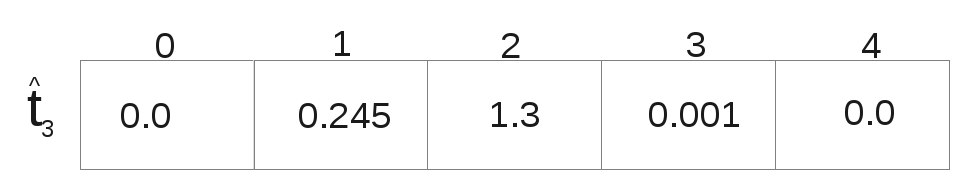
\includegraphics{immagini/test/tBFSmodoA}
 \caption{Esempio del vettore di trustrank calcolato su una porzione di grafo a cui viene assegnato il valore 0.0 ai nodi non visitati.}
 \label{fig:tBFSmodoA}
\end{figure}
\begin{figure}
\centering
 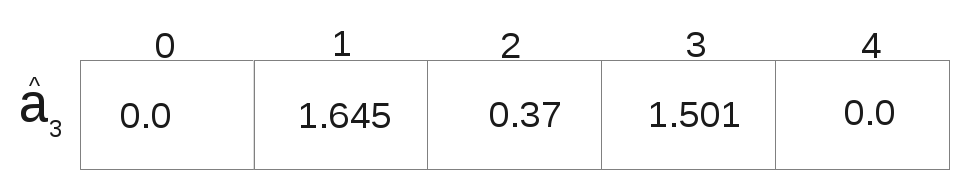
\includegraphics{immagini/test/aBFSmodoA}
 \caption{Esempio del vettore di anti-trust rank calcolato su una porzione di grafo a cui viene assegnato il valore 0.0 ai nodi non visitati.}
 \label{fig:aBFSmodoA}
\end{figure}

I test saranno, quindi, cosi strutturari:
\begin{itemize}
 \item Test numero 1. Si confronta \textit{trustrank} sul grafo completo con \textit{trustrank} calcolato su una porzione di grafo. Lo stesso si fa per \textit{anti-trust ran}.
 \item Test numero 2. Si confrontano i solo nodi etichettati spam del vettore di  \textit{trustrank} sul grafo completo con  i soli nodi etichettati spam del vettore di \textit{trustrank} calcolato su una porzione di grafo. Nel caso di \textit{anti-trust rank} si  confrontano i nodi etichettati come non spam.
 \item Test numero 3. Si calcola \textit{trustrank} sul grafo completo ottenuto eseguendo la visita partendo da un nodo \(s\) e si confronta con \textit{trustrank} eseguito a ogni passo delle visita ma si imposta un seedset diverso formato dagli ultimi \(n\) nodi della vista. Viene applicato lo stesso metodo per \textit{anti-trust rank}.
 \item Test numero 4. Viene rieseguito il \textit{test numero 3} ma con il fattore di attenuazione \(\alpha\), utilizzato nel calcolo di \textit{trustrank} e \textit{anti-trust rank} impostato a 0.0005.
 \item Test numero 5. Si esegue la BFS a partire dal nodo \(s\) e per ogni passo si calola la media dei valori di \textit{trustrank} dei soli nodi che sappiamo essere non spam e la media dei valori di \textit{Trustrank} dei soli nodi spam. Quindi si calcola la differenza tra le due medie. Lo stesso metodo verrà applicato per l'analisi dell'algoritmo di \textit{anti-trust rank}.
  \item Test numero 6. Si riesegue il \textit{test numero 5} ma invece di usare dei valori temporani di \textit{trustrank} e \textit{anti-trust rank} a ogni passo della visita per calcolare le relative medie, si utilizzano i valori finali di \textit{trustrank} e \textit{anti-trust rank} calcolati sull'intero grafo.
 \end{itemize}
 
\section{Test 1}
 Questo test calcola la distanza, tramite della Tau di Kendall denominata \(T_t\), tra il vettore \(t\) di \textit{trustrank} ricavato sull'intero grafo e il vettore \(\hat{t}_i\) di \textit{trustrank} calcolato sul grafo ricavato dai nodi visitati lungo una visita in ampiezza con nodo sorgente \(s\). Inoltre viene eseguto lo stesso procedimento per quanto riguarda \textit{anti-trust rank} ovvero si calcolano le distanze, sempre utlizzando una Tau di Kendall che denomineremo \(T_a\),  tra il vettore di \(a\) di \textit{anti-trust rank} ottenuto dal grafo completo e il vettore \(\hat{a}_i\)  caloato sul grafo ricavato dai nodi visitati lungo  un visita in ampiezza con nodo sorgente \(s\). Dal dataset sono impostati come nodo sorgente della BFS due nodi: il nodo 62 etichettato come non spam e il nodo 112 etichettato come spam. Inoltre per il calcolo di \textit{trustrank} sull'intero grafo viene utilizzato come seedset l'insieme di pagine del dataset WEBSPAM-UK2007 etichettate come non spam mentre per il 
calcolo di \textit{trustrank} sul grafo ottenuto dai nodi visitati durante la BFS il seedset sarà formato dalle pagine visitate che sono etichettate come non spam nel dataset WEBSPAM-UK2007. Per il calolo di \textit{anti-trust rank} sull'intero grafo, invece, il seedset sarà composto dalle pagine etichettate come spam nel dataset WEBSPAM-UK2007 mentre il seedset di \textit{anti-trust rank} calcolato sul grafo ottenuto dai nodi visitati dalla BFS sarà formato dai soli nodi visitati che sono etichettati come spam.

In figura \ref{fig:test1trustModoB62} e in figura \ref{fig:test1trustModoB112} sono rappresentati rispettivamente i grafici delle Tau di Kendall \(T_{t62}\) e \(T_{t112}\), per il cacolo delle distanze tra il vettore \(t\) calcolato sull'intero grafo e il vettore \(\hat{t}_i\) calcolato sul grafo ottenuto dai nodi visitati lungo una visita in ampiezza con nodo sorgente nel primo caso 62 e nel secondo con nodo sorgente 112.  Sull'asse delle ascisse è rappresentato il numero di nodi che sono stati visitati attraverso la BFS e quindi il numero di nodi del grafo su cui viene calcolato \(\hat{t}_i\) dove \(i\) è appunto il numero di nodi presi in considerazione, mentre sull'asse delle ordinate è rappresentato il valore della Tau di Kendall tra il vettore \(t\) e \(\hat{t}_i\).\\
I due grafici sono molto simili è quindi il calcolo di \(\hat{t}_i\) non dipende dal nodo da cui sorgente della visita in ampiezza. Il valore di Tau di Kendall uguale ad 1 si ha quando la BFS ha visitato solamente il nodo di partenza, quindi  il vettore \(t\) avrà un solo indice (che fa riferimento al nodo sorgente) e il vettore \(\hat{t}_1\) avrà anche esso un solo indice (il quale fa riferimento al nodo sorgente) perciò  la Tau di Kendall tra i due vettori ritorna un valore uguale ad 1; è facile intuire che questo valore non è influente nella valutazione ma è un risultato dovuto al fatto che si calcolcola la Tau di Kendall su vettori composti da un unico elemento, quindi i valori significativi sono i successici.\\
Dopo che la visita entra in profondità il valore delle Tau di Kendall \(T_{t62}\) e \(T_{t112}\)  scendono dastricamente a circa 0.7 per poi aumentare fino a circa 1 tanto più la visita in ampiezza scopre i nodi del grafo; tale comportamento indica che la distanza tra il vettore \(t\) e \(\hat{t}_i\) dipende dal numero di nodi visitati tramite la visita in ampiezza. 

 \begin{figure}
\centering
 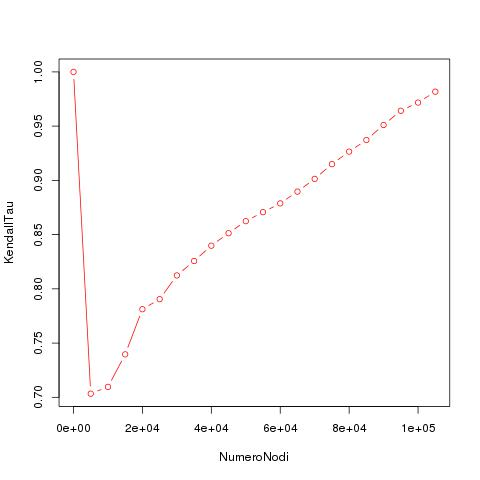
\includegraphics[height=9cm]{immagini/test1/trustranktestMode1_62}
 \caption{Test numero 1 (trustrank, 62). Calcolo della distanza dei vettori tra trustrank calcolato sull'intero grafo e trustrank calcolato sul grafo ricavato dai nodi visitati lungo una BFS partendo dal nodo 62.}
 \label{fig:test1trustModoB62}
\centering
 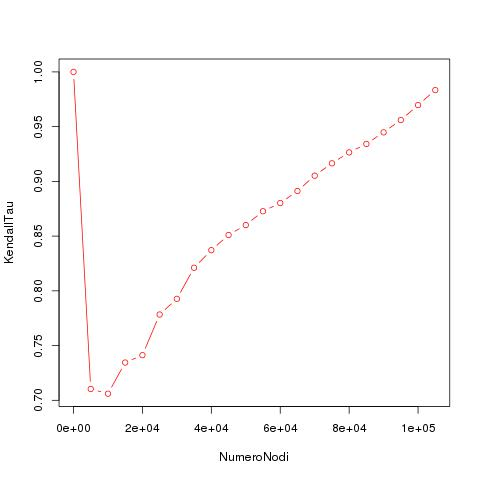
\includegraphics[height=9cm]{immagini/test1/trustranktestMode1_112}
 \caption{Test numero 1 (trustrank, 112). Calcolo della distanza dei vettori tra trustrank calcolato sull'intero grafo e trustrank calcolato sul grafo ricavato dai nodi visitati lungo una BFS partendo dal nodo 112.}
 \label{fig:test1trustModoB112}
\end{figure}

Eseguendo lo stesso test per valutare la distanza tra il vettore \(a\) di \textit{anti-trust rank} calcolato sull'intero grafo e il vettore \(\hat{a}_i\) calcolato sul grafo ottenuto dai nodi visitati durante una visita in ampiezza si nota che i risultati sono presocchè uguali ai precedenti due test. In particolare in figura \ref{fig:test1antitrustModoB62} è rappresentato il grafico della Tau di Kendal \(T_{a62}\) che mette a confronto il vettore \(a\) con il vettore \(\hat{a}_i\) dove la BFS ha come nodo sorgente 62 mentre in figura \ref{fig:test1antitrustModoB112} è rappresentato il grafico della Tau di Kendall \(T_{a112}\) che mette a confronto il vettore \(a\) con il vettore \(\hat{a}_i\) dove la BFS ha nodo sorgente 112; sull'asse delle ascisse è rappresentao il numero di nodi che sono visitati durante la BFS mentre sulle ordinate il corrispondente valore di Tau di Kendall tra il vettore di \(a\) calcolato sull'intero grafo e il vettore \(\hat{a}_i\) calcolato sul grafo ricavato dai nodi visitati 
attraverso una BFS a diversi passi, quindi \(i\) sarà uguale al numero dei nodi visitati ad un certo istante. Rispetto al test di \textit{trustrank} usando \textit{anti-trust rank} si nota che i grafici (senza considerare il primo valore per lo stesso motivo dei due test precedenti) hanno un andamento quasi logaritmico dove si ha come valore iniziale di Tau di Kendall 0.75 e come utlimi valori (stazionari) 0.95. Infatti un fattore evidente è che la Tau di Kendall tende a non superare il 0.95 per gli ultimi nodi incontrati nella BFS.

 \begin{figure}
\centering
 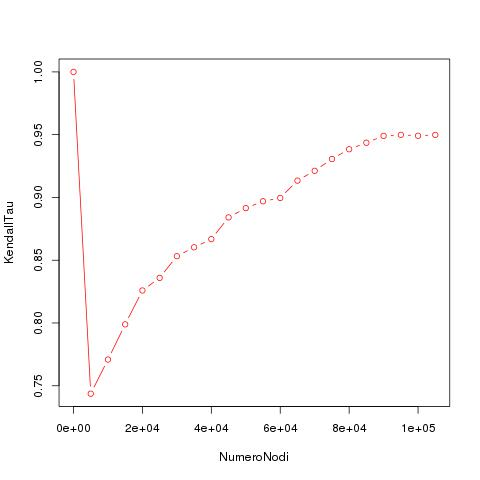
\includegraphics[height=9cm]{immagini/test1/antiTrustrankTestMode1_62}
 \caption{Test numero 1 (anti-trust rank, 62). Calcolo della distanza dei vettori tra anit-trust rank calcolato sull'intero grafo e anti-trust rank calcolato sul grafo ricavato dai nodi visitati lungo una BFS parteneo dal nodo 62.}
 \label{fig:test1antitrustModoB62}
\centering
 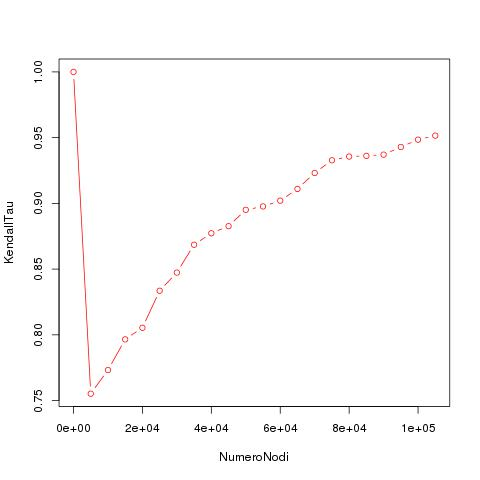
\includegraphics[height=9cm]{immagini/test1/antiTrustrankTestMode1_112}
 \caption{Test numero 1 (anti-trust rank, 112). Calcolo della distanza dei vettori tra anit-trust rank calcolato sull'intero grafo e anti-trust rank calcolato sul grafo ricavato dai nodi visitati lungo una BFS parteneo dal nodo 112.}
 \label{fig:test1antitrustModoB112}
\end{figure}

In figura \ref{fig:test1coplot62} sono riportati in un unico grafico i grafici rappresentati in figura \ref{fig:test1trustModoB62} relativo a \(T_{t62}\) e del  grafico \ref{fig:test1antitrustModoB62} relativo a \(T_{a62}\); in rosso è rappresentato il grafico raffigurante \(T_{t62}\) tra \textit{trustrank} calcolato sull'intero grafo e \textit{trustrank} calcolato sul grafo ottenuto dai nodi visitati a diversi passi di una BFS con nodo sorgente 62 mentre in verde è rappresentato il grafico  rappresentante \(T_{a62}\) tra \textit{anti-trust rank} calcolato sull'intero grafo e \textit{anti-trust rank} calcolato sul grafo ottenuto dai nodi visitati a diversi passi di una BFS con nodo sorgente 62. Quello che evince è che \(T_{a62}\) applicata al vettore \(a\) e \(\hat{a}_i\) cresce più velocemente rispetto a \(T_{t62}\) applicata a   \(t\) e \(\hat{t}_i\) ma che dopo la visita di circa 80000 \(T_{t62}\) assume valori più alti rispetto a \(T_{a62}\); infatti come avevamo detto i valori di \(T_{a62}\) tendono a 
fermarsi intorno a 0.95.\\
Tale comportamento tra \(T_{t62}\) e \(T_{a62}\) indica perciò che \textit{trustrank} eseguito online è più efficace di \textit{anti-trust rank} nel approssimare il loro comportamento offline ma solo dopo che sono stati visitati molti nodi mentre \textit{anti-trust rank} online riesce ad approssimare bene il suo comportamento anche se eseguito su un numero esiguo di nodi dell'intero grafo. Quindi  tra \textit{trustrank} e \textit{anti-trust rank} il miglior metodo per essere utilizzato in modalità online è \textit{anti-trust rank} perché tende ad approssimare fin da subito il comportamento offline anche avendo pochi nodi. Infatti il grafico in figura \ref{fig:test1coplot62} indica che \textit{anti-trust rank} eseguito durante la fase di crawling ritorna un vettore dove i valori tendono ad avvicinarsi rapidamente ai valore del vettore se \textit{anti-trust rank} fosse eseguito in modalità offline.\\
Le stesse valutazioni valgono tra il confronto dei due grafici in figura \ref{fig:test1trustModoB112} relativo a \(T_{t112}\) e \ref{fig:test1antitrustModoB112}  relativo a \(T_{a112}\) illustrato in figura \ref{fig:test1coplot112} dove in rosso è rappresentata la Tau di Kendall \(T_{t112}\) tra \textit{trustrank} calcolato sull'intero grafo e \textit{trustrank} calcolato sul grafo ottenuto dai nodi visitati a diversi passi di una BFS con nodo sorgente 112 mentre in verde è rappresentato il la Tau di Kendall \(T_{a112}\) tra \textit{anti-trust rank} calcolato sull'intero grafo e \textit{anti-trust rank} calcolato sul grafo ottenuto dai nodi visitati a diversi passi di una BFS con nodo sorgente 112. Come si nota anche in questo caso \textit{anti-trust rank} online riesce ad approssimare bene con  pochi nodi, rispetto al grafo completo, il comportamento offline differentemente a \textit{trustrank} che non riesce ad avere le stesse prestazioni tranne quando si hanno molti nodi (nel grafico in particolare piu di 
80000) in questo caso le prestazioni di \textit{trustrank} superano quelle di \textit{anti-trust rnak}. Tali deduzioni si evincono dal fatto che \(T_{a112}\) cresce più rapidamente rispetto a \(T_{t112}\) ma dopo circa 80000 \(T_{a112}\) cresce più lentamente rispetto a \(T_{t112}\) che raggunge valori più alti.

 \begin{figure}
\centering
 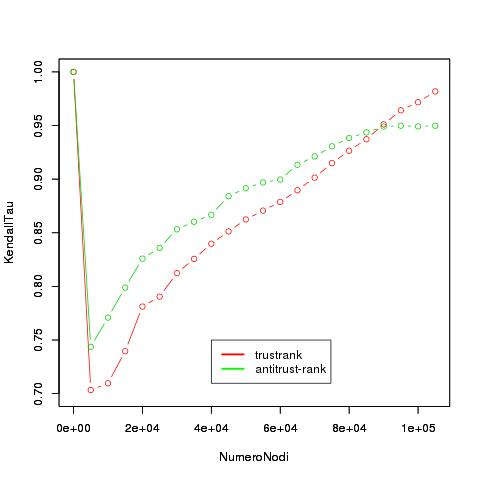
\includegraphics[height=9cm]{immagini/test1/coplotTrustAnti_62}
 \caption{Plotting del grafico \ref{fig:test1trustModoB62} e del  grafico \ref{fig:test1antitrustModoB62}}
 \label{fig:test1coplot62}
\centering
 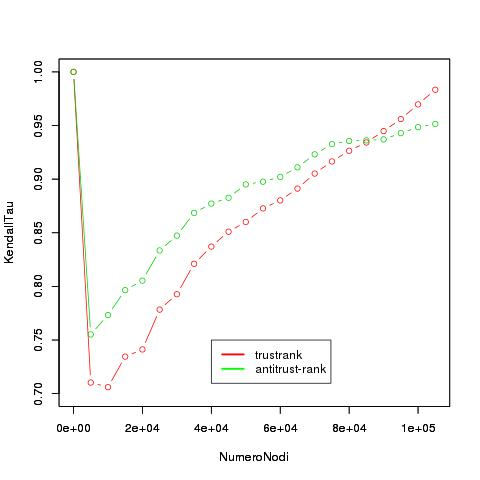
\includegraphics[height=9cm]{immagini/test1/coplotTrustAnti_112}
 \caption{Plotting del grafico \ref{fig:test1trustModoB112} e del  grafico \ref{fig:test1antitrustModoB112}}
 \label{fig:test1coplot112}
\end{figure}

\section{Test 2}
Il test consiste nel valutare la distanza tra due vettori, utilizzanto una Tau di Kendall \(T_t\), il vettore \(t\) di \textit{trustrank} calcolato sull'intero grafo e il vettore \(\hat{t}_i\) calcolato sul grafo ottentuto dai nodi visitati durante un visita in ampiezza; quindi la distanza viene calcolata ogni qual volta il numero di indici, del vettore \(\hat{t}_i\), a cui è possibile associare un valore aumenta  di un certo intervallo ovvero  quando la BFS visita un intervallo di nodi stabilito adentrandosi sempre di più nel grafo. Il test cosi descritto è simile al \textit{Test numero 1} ma differentemente del precedente in questo test nel determinare la distanza tra i due vettori si esaminano i soli indici dei vettori \(t\) e \(\hat{t}_i\) che fanno riferimento ai nodi etichettati come spam. Ugualmente il test viene effettuato per valutare \textit{anti-trust rank} ma in questo caso vengono confrontati, tramite la Tau di Kendall \(T_a\), i soli nodi indici dei due vettori \(a\) e \(\hat{a}_i\) che fanno 
riferimento a nodi etichettati come non spam.

Anche per questo test nella valutazione di \textit{trustrank} è stato usato come seedset l'insieme dei nodi etichettati non spam del dataset WEBSPAM-UK2007 mentre per \textit{anti-trustrank} è stato usto come seedset l'insieme dei nodi spam del dataset WEBSPAM-UK2007.

\begin{figure}
\centering
 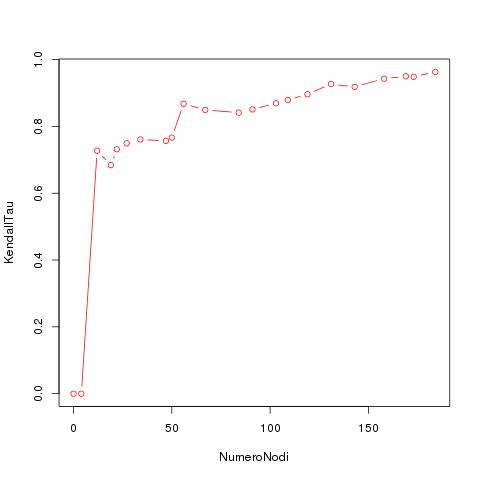
\includegraphics[height=9cm]{immagini/test2/trustrankBadNodesTestMode1_62}
 \caption{Test numero 2 (trustrank, 62). Calcolo della distanza dei vettori tra trustrank calcolato sull'intero grafo e trustrank calcolato sul grafo ricavato dai nodi visitati lungo una BFS partendo dal nodo 62 prendendo in considerazione i soli nodi spam. }
 \label{fig:test2trustModoB62}
\centering
 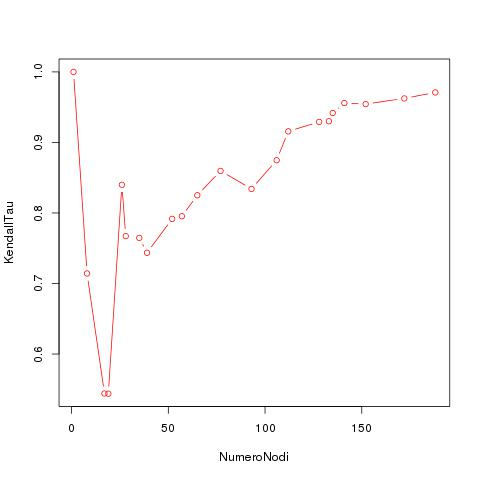
\includegraphics[height=9cm]{immagini/test2/trustrankBadNodesTestMode1_112}
 \caption{Test numero 2 (trustrank, 112). Calcolo della distanza dei vettori tra trustrank calcolato sull'intero grafo e trustrank calcolato sul grafo ricavato dai nodi visitati lungo una BFS partendo dal nodo 112 prendendo in considerazione i soli nodi spam.}
 \label{fig:test2trustModoB112}
\end{figure}

In figura \ref{fig:test2trustModoB62} è rappresentato il grafico della Tua di Kendall \(T_{t62}\) tra gli indici spam dei vettori \(t\) e \(\hat{t}_i\)  di tale dove il nodo sorgente della visita in ampiezza, con cui viene ricavato il grafo temporaneo sui cui viene calcolato \(\hat{t}_i\) è 62. Sull'asse delle ascisse è rappresentato il numero di nodi spam visitati durante la visita in ampiezza e sull'asse delle ordinate la Tau di Kendall \(T_{t62}\) calcolata a ogni intervallo di nodi visitati (compresi nodi spam e non spam).\\
Al primo passo, come per il \textit{test numero 1}, quando la visita in ampiezza ha visitato il solo nodo sorgente ci si aspetta che il vaore di \(T_{t62}\) sia  1 in quanto i vettori \(t\) e \(\hat{t}_i\) dovrebbero essere composti dal solo nodo visitato al primo passo (e quindi il nodo sorgente 62).  Ma dal momento che si stanno prendendo i soli nodi etichettati spam, il nodo 62 essendo etichettato non spam  viene scartato e quindi il vettore \(t\) e \(\hat{t}_i\) saranno vuoti e quindi \(T_{t62}\) al primo passo assume valore 0. Dopo di che con l'avanzanto della visita in ampiezza e appena questa incomincia ad incontrare nodi spam l'andamento del grafico cresce rapidamente fino a circa 0.7 per poi variare gradualemnte fino a circa 1.0.

\begin{figure}
\centering
 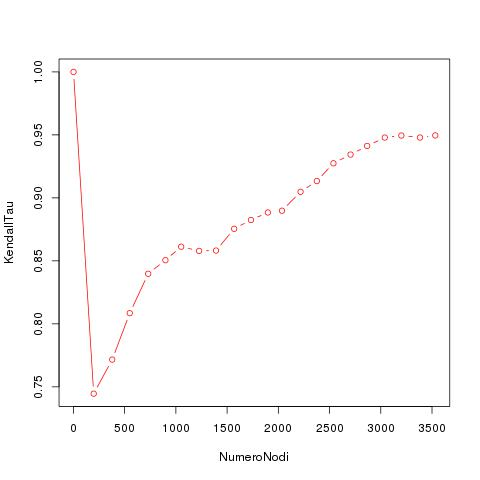
\includegraphics[height=9cm]{immagini/test2/antiTrustraktGoodNodesTestMode1_62}
 \caption{Test numero 2 (anti-trust rank, 62). Calcolo della distanza dei vettori tra anti-trust rank calcolato sull'intero grafo e anti-trust rank calcolato sul grafo ricavato dai nodi visitati lungo una BFS partendo dal nodo 62 prendendo in considerazione i soli nodi non spam. }
 \label{fig:test2antitrustModoB62}
\centering
 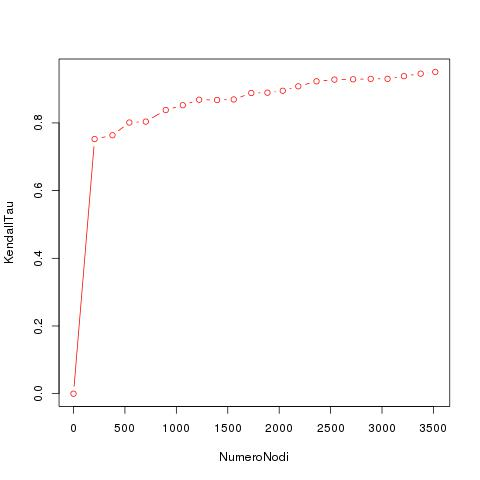
\includegraphics[height=9cm]{immagini/test2/antiTrustraktGoodNodesTestMode1_112}
 \caption{Test numero 2 (anti-trust rank, 62). Calcolo della distanza dei vettori tra anti-trust rank calcolato sull'intero grafo e anti-trust rank calcolato sul grafo ricavato dai nodi visitati lungo una BFS partendo dal nodo 112 prendendo in considerazione i soli nodi non spam. }
 \label{fig:test2antitrustModoB112}
\end{figure}

Il grafico della Tau di Kendall \(T_{t112}\)  calcolata  per ogni intervallo di nodi visitati tramite la visita in ampiezza con nodo sorgente 112 è rappresentato in figura \ref{fig:test2trustModoB112}.  Sull'asse delle ascisse è rappresentato il numero dei soli nodi spam visitati tramite la visita in ampiezza e sull'asse delle ordinate la Tau di Kendall \(T_{t112}\) calcolata a ogni intervallo di nodi visitati (compresi nodi spam e non spam).\\
In questo caso il primo valore della Tau di Kendall \(T_{t112}\) è 1 perché  il nodo sorgente 112 essendo spam verrà preso in considerazione nella valutazine, perciò i vettori \(t\) e \(\hat{t}_i\) saranno composti da un unico indice che fa riferimento al nodo 112 e la Tau di Kendall applicata a vettori composti da un solo elemento è uguale a 1. Ma con l'avanzamento della visita in ampiezza l'andamento della Tau di Kendall \(T_{t112}\) calcolata su \(t\) e \(\hat{t}_i\) varia tra circa 0.5 e 1.

Lo stesso test è stato applicato per valutare \textit{anti-trust rank}; in figura \ref{fig:test2antitrustModoB62} è illustrato il grafico relativo alla Tau di Kendall \(T_{a62}\) per il calcolo della distanza tra il vettore \(a\) e il vettore \(\hat{a}_i\) prendendo in considerazione i soli nodi non spam e la visita in ampiezza con nodo sorgente 62, mentre in figura \ref{fig:test2antitrustModoB112} è illustrato il grafico relativo alla Tau di Kendall \(T_{a112}\) per il calcolo della distanza tra il vettore \(a\) e il vettore \(\hat{a}_i\) prendendo in considerazione i soli nodi non spam e la visita in ampiezza con nodo sorgente 112. Sull'asse delle ascisse è rappresentato il numero dei soli nodi non spam incontrati tramite la visita in ampiezza tra tutti i nodi visitati e sull'asse delle ordinate la Tau di Kendall calcolato a ogni intervallo di nodi visitati.\\
Nel primo grafico si nota che a differenza del test su \textit{trustrank} con nodo sorgente, della BFS, 62 il primo valore della Tau di Kendall \(T_{a62}\), ovvero quando la visita in ampiezza ha visitato il solo nodo sorgente e quindi il grafo temporaneo è formato dal solo nodo 62, è 1 perchè in questo caso si esaminano i nodi non spam e tale nodo essendo non spam non viene rigettatto ma viene esaminato e quindi i vettori \(a\) e\(\hat{a}_i\) avranno un solo valore relativo al nodo 62 e perciò la Tau di Kendall \(T_{a112}\) al primo passo sarà 1. Con l'aumentare dei nodi visitati i valori di \(T_{a62}\) variano da circa 0.75 a 0.95.

Il secondo grafico mentre ha come primo valore della Tau di Kendall \(T_{a112}\) uguale a 0, questo perchè il grafo temporaneo è formato al primo passo èdal solo nodo 112 e quindi dal momento che 112 è un nodo spam viene rigettato e non esaminato. Perciò in questo caso sia il vettore \(a\) che il vettore \(\hat{a}_i\) avranno lunghezza zero fino al momento in cui la visita in ampiezza non incotra dei nodi non spam infatti nei passi successivi il grafico varia da circa 0.8 a circa 1.

\section{Test 3}
Questo test è stato ideato in modo da creare una situazione avversariale e mettere in difficoltà gli algoritmi di \textit{trustrank} e \textit{anti-trust rank} durante la loro esecuione in modalità online. Ovvero si è pensato di simulare il caso in cui il seedset che viene utilizzato dagli algoritmi (il quale va a definire la distribuzione di probabilità rappresentata dal vettore di preferenza dell'algoritmo di \textit{pagerank}) sia totalmente sbagliato e vedere i risultati che questo comporta nell'esecuzione in modalità online.

Il test, quindi, consiste (per la valutazione di \textit{trustrank}) nel eseguire una visita in ampiezza \(v_1\) da un nodo sorgente \(s\) e calcolare \textit{trustrank} sul grafo composto da tutti i nodi visitati alla fine della visita (che denomineremo \(t_v\)) dove il seedset \(S\) usato dall'algoritmo è composto dagli ultimi \(n\) nodi visitati da \(v_1\); dopodiché  si riesegue una seconda visita in ampiezza \(v_2\) con nodo sorgente \(s\) e si calcola \textit{trustrank}, per ogni intervallo di nodi visitati, sul grafo ottenuto da questi nodi (che denomineremo \(\hat{t}_i\)) con seedset \(S\) formato dagli ultimi \(n\) nodi visitati tramite la visita in ampiezza \(v_1\). Il numero di \(n\) nodi utilizzato è 3776 come la grandezza dell'insieme delle pagine eticchettate non spam nel dataset WEBSPAM-UK2007. Quindi si calcola la Tau di Kendall \(T_t\) tra il vettore \(t_v\) e il vettore \(\hat{t}_i\) ad ogni intervallo di nodi che vengono visitati tramite la visita in ampiezza \(v_2\).\\
Lo stesso test è stato applicato per valutare \textit{anti-trust rank}. In questo caso si esegue una visita in ampiezza \(v_1\) da un nodo sorgente \(s\) e viene calcolato \textit{anti-trust rank} sul grafo composto da tutti i nodi visitati alla fine della visita (denominato \(a_v\)) e il seedset \(S\) utilizzato per il calcolo di \(a_v\) è composto dagli ultimi \(n\) nodi visitati da \(v_1\); successivamente si riesegue una seconda visita in ampiezza \(v_2\) con nodo sorgente \(s\) e si calcola \textit{anti-trust rank}, per ogni intervallo di nodi visitati, sul grafo ottenuto da questi nodi (che denomineremo \(\hat{a}_i\)) dove il seedset usato dall'algoritmo di \textit{anti-trust rank} è formato come prima dai nodi dell'insieme \(S\). Infine  viene calcolata la Tau di Kendall \(T_t\) tra il vettore \(a_v\) e il vettore \(\hat{a}_i\) ogni intervallo di nodi che vengono visitati tramite la visita in ampiezza. Anche in questo caso il numero di nodi \(n\) scelti come seedset sarà 3776.\\
Durante il calcolo di \(\hat{t}_i\) e di \(\hat{a}_i\), sul grafo temporaneo ottenuto dai nodi lungo la visita in ampiezza \(v_2\), finché la visita non incontrerà i nodi facenti parte dell'insieme \(S\) il vettore di preferenza con cui si calcolerà \(\hat{t}_i\) e \(\hat{a}_i\) sarà una distribuzione uniforme, il che siginifica che nel caso di \textit{trustrank} sarà come calcolare \textit{pagerank} mentre nel caso di \textit{anti-trustrank} sarà come calcolare \textit{pagerank} trasposto. Nel momento in cui la visita in ampiezza incomincerà ad incotrare qualche nodo dell'insieme \(S\) allora il vettore di preferenza verrà manipolato con una distribuzione personalizzata basata sui nodi appartenenti all'insieme \(S\) che sono stati visitati. 


In figura \ref{fig:test3coplotTrustAntiModeB62} è rappresentato il grafico del test eseguito per valutare \textit{trustrank} e \textit{anti-trust rank}; in particolare è raffigurata la Tau di Kendall \(T_{t62}\) tra il vettore \(t_v\) e il vettore \(\hat{t}_i\) calocolato sul grafo temporaneo ricavato dalla visita in ampiezza \(v_2\) con nodo sorgetne 62, e la Tau di Kendall \(T_{a62}\) tra il vettore \(a_v\) e il vettore \(\hat{a}_i\) calocolato sul grafo temporaneo ricavato dalla visita in ampiezza \(v_2\) con nodo sorgente 62. Sull'asse delle ascisse è rappresentato il numero di nodi visitati tramite la visita \(v_2\) mentre sull'asse delle ordinate il valore delle Tau di Kendall \(T_{t62}\) e \(T_{a62}\). In rosso è illustrato il grafico della Tau di Kendall \(T_{t62}\)  mentre in verde è rappresentato l'andamento della Tau di Kendall \(T_{a62}\).\\ Il primo valore delle Tau di Kendall \(T_{t62}\) e \(T_{a112}\) è 1 per il fatto che la vista \(v_2\) ha incontrato il solo nodo sorgente percio al passo uno 
il grafo temporaneo sarà composto dal solo nodo 62 e i vettori \(t_v\) e \(\hat{t}_i\), nel caso di \(T_{t62}\), \(a_v\) e \(\hat{a}_i\), nel caso di \(T_{a62}\), saranno composti da un solo indice relativo al nodo sorgente 62 e quindi le Tau di Kendall ritorneranno valore 1.
\begin{figure}
\centering
 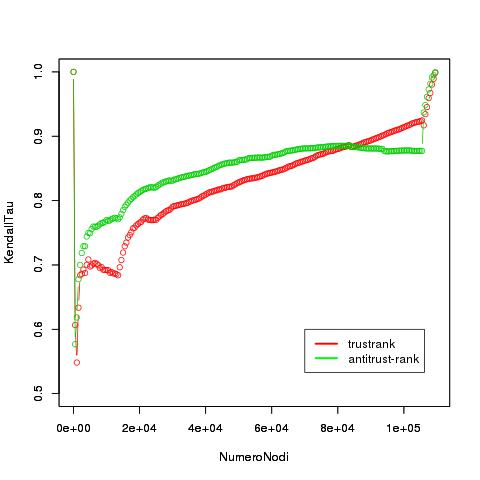
\includegraphics[height=9cm]{immagini/test3/coplotTrustAnti_Mode1_set3776_62}
 \caption{Test numero 3 . In rosso, calcolo della Tau di Kendall  tra il vettore $t_v$ e il vettore $\hat{t}_i$ per ogni intervallo di nodi visitati della BFS partendo dal nodo 62. In verde calcolo della Tau di Kendall tra il vettore $a_v$ e il vettore $\hat{a}_i$ per ogni intervallo di nodi visitati della BFS partendo dal nodo 62}
 \label{fig:test3coplotTrustAntiModeB62}
\end{figure}
Con l'avanzare della visita in ampiezza \(v_2\) i valori della Tau di Kendall \(T_{t62}\) incominciano da circa 0.55, dopo aver visitato il primo nodo, e salgono gradualmente a circa 0.9 dopo aver visitato 105790 nodi. Dal momento che dal nodo 62 si riescono a visitare 109566 nodi su 114529 totali del grafo e dal momento che il seedset \(S\) è formato dagli ultimi 3776 nodi della visita in ampiezza \(v_2\) allora fino a 109570 il vettore di preferenza con cui è calcolato \(\hat{t}_i\) è uguale a una distribuzione uniforme mentre dopo aver visitato 109570 nodi il vettore di preferenza cambia e verrà manipolato tramite i nodi incontrati facenti parte dell'insieme \(s\). Quindi dopo aver visitato 109570 nodi i valori della Tau di Kendall \(T_{t62}\) salgono rapidamente fino a toccare 1 quando il seedset con cui è calcolato \(\hat{t}_i\) è formato completamente da tutti i nodi in \(S\). La stesso comportamento è riscontrabile per la Tau di Kendall \(T_{a62}\). Un altro importante dato che si evince dal 
comportamento della Tau di Kendall \(T_{t62}\) e della Tau di Kendal \(T_{a62}\) è che \(T_{a62}\) cresce più rapidamente rispetto alla Tau di Kendall \(T_{t62}\) che cresce lentamente ma tale comportamento cambia dopo che \(v_2\) ha incontrato circa 80000 nodi. Quindi questo vuol dire che \textit{anti-trust rank} è meno dipendente dal vettore di preferenza che gli viene passato rispetto a \textit{trustrank} almeno fino a quando si ha un grafo temporane molto piccolo rispetto al grafo completo e perciò anche se si usasse \textit{anti-trust rank} in modalità online con un seedset poco pertinente questo riuscirebbe a produrre subito dei risultati molto vicini a quelli calcolati da \textit{anti-trust rank} sull'intero grafo con un altro seedset. Mentre \textit{trustrank} non riesce ad approsimare bene tale comportamento rispetto ad \textit{anti-trust rank} fino a quando non sia calcolato sul grafo temporaneo formato da almeno il 60\% dei nodi dell'intero grafo.

\section{Test 4}
Questo test è molto simile al \textit{test numero 3} dove, però, il fattore di attenuazione \(\alpha\) con cui viene calcolato il vettori \(t_v\) di \textit{trustrank} ottenuto dall'analisi del grafo ottenuto al termine della visita in ampiezza \(v_1\) con nodo sorgente \(s\) e \(\hat{t_i}\) otteunto dall'analisi del grafo temporaneo ricavato ad ogni intervallo nodi visitati tramite la visita \(v_2\) con nodo sorgente \(s\) è uguale a 0.005. Ed inoltre il seedset con cui sono eseguiti \textit{trustrank} e \textit{anti-trust rank} è composto dagli ultimi \(n\) (dove \(n\) è ugale a 3776) nodi incontrati tramite la visita in ampiezza \(v_1\). Lo stesso metodo è stato applicato per analizzare \textit{anti-trust rank} dove \(a_v\) indica il grafo ottenuto al termine della visita in ampiezza \(v_1\) con nodo sorgente \(s\) e \(\hat{a}_i\) indica il grafo temporaneo ottenuto ad ogni intervallo di nodi visitati traminte la visita in ampiezza \(v_2\) con nodo sorgente \(s\). Il nodo sorgente è 62.\\
Il fattore \(\alpha\) impostato ad un valore molto vicino allo 0 aumenta la probabilità che \textit{trustrank} o \textit{anti-trust rank} scelgano di privileggiare la distribuzione descritta dal vettore di preferenza invece di seguire un semplice camminata sul grafo (per maggiori chiarimenti si consiglia di leggere il paragrafo \ref{sub:esogeno} dove è descritto \textit{Pagerank}).
\begin{figure}
 \centering
 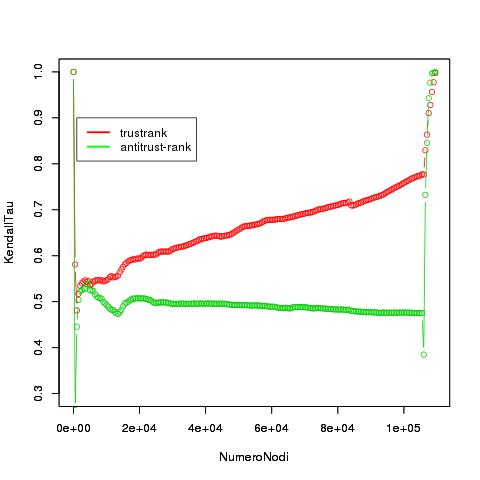
\includegraphics[height=9cm]{immagini/test4/coplotTrustAnti_Mode1_set3776_62_alpha0005}
  \caption{Test numero 4 . In rosso, calcolo della Tau di Kendall tra il vettore $t_v$ e il vettore $\hat{t}_i$, dove $\alpha$ è impostato a 0.005. In verde calcolo della Tau di Kendall tra il vettore $a_v$ e il vettore $\hat{a}_i$, dove $\alpha$ è impostato a 0.005.}
 \label{fig:test4coplotTrustAntiModeB620005}
\end{figure}

In figura \ref{fig:test4coplotTrustAntiModeB620005} è illustrato il grafico della Tau di Kendall \(T_{t62}\) tra \(t_v\) e \(\hat{t}_i\) (in rosso)  e della Tau di Kendall \(T_{a62}\) tra \(a_v\) e \(\hat{a}_i\) (in verde). Sull'asse delle ascisse è rappresentato il numero di nodi visitati tramite la visita \(v_2\) mentre sull'asse delle ordinate il valore delle Tau di Kendall \(T_{t62}\) e \(T_{a62}\). Come si nota dal grafico dopo la \(T_{t62}\) tende a crescere regolarmente fino a circa 109570 dopo dopodiché quando la visita \(v_2\) incontra i primi nodi \(S\) allora \(\hat{t}_i\) tende ad avere valori sempre più simili a \(t_v\) fino ad arrivare a 1 quando tutti i nodi in \(S\) sono stati visitati tramite \(v_2\) e quindi \(\hat{t_i}\) avra come seedset l'insieme \(S\). Differentemente \(T_{a62}\) risente maggiormente del fatto che \(a_v\) e \(\hat{a}_i\) sia stato calcolato con un fattore di attenuazione uguale a 0.005, infatti il grafico mostra come quanto più la visita in ampiezza \(v_2\) entra in 
profondità i due vettori \(a_v\) e \(\hat{a}_i\) siano sempre più distanti e solo dopo che \(v_2\) incomincia ad incontrare i nodi \(S\) e il seedset con cui \(\hat{a}_i\) viene calcolato è rimpiazzato dai nodi visitati in \(S\), la Tau di Kendall \(T_{a62}\) incomincia a crescere fino ad arrivare a 1 quando tutti i nodi  in \(S\) sono stati visitati.

%inserire raggionamento perchè si ottengono i risultati nel test3 e test4, forse è dovuto al fatto che antitrustrank è calcolato sul grafo trasposto

\section{Test 5}
Questo test consiste nel calcolare, ad ogni passo di una visita in ampiezza  con nodo sorgente \(s\), \textit{trustrank} \(\hat{t}_i\) sul grafo temporaneo ottenuto dai nodi visitati sull'intero grafo e dopodiché calcolare la media \(Mb_t\) dei valori di \textit{trustrank} dei nodi etichettati non spam e la media \(Ms_t\) dei valori di \textit{trustrank} dei nodi etichettati spam ed infine ottenere la differenza tra le due medie \(Diff_t\). Quindi:
\begin{equation}
 Diff_t = Mb_t-Ms_t
\end{equation}
Questa differenza verra calcolata per ogni intervallo di nodi visitati tramite la visita in ampiezza. Lo stesso test è applicato per analizzare \textit{anti-trust rank} perciò ad ogni intervallo di nodi visitato  dalla visita in ampiezza con nodo sorgente \(s\) viene calcolato il vettore \(\hat{a}_i\)  di \textit{anti-trust rank}  calcolato sul grafo temporaneo ottenuto dai nodi della visitala differenza e succesvamente vien calcolata la diffenreza \(Diff_a\) tra le media \(Mb_a\) dei valori di \textit{anti-trust rank} dei nodi non spam ,e la media \(Ms_a\) dei valori di \textit{anti-trust rank} dei nodi etichettati spam. Quindi:
\begin{equation}
 Diff_a=Mb_a-Ms_a
\end{equation}

 
\begin{figure}
 \centering
 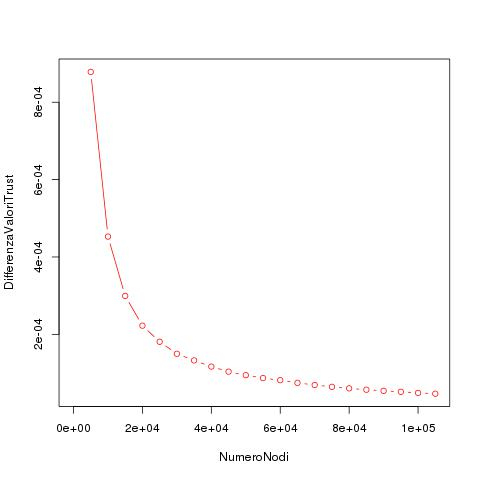
\includegraphics[height=9cm]{immagini/test5/averageTest_trust_62}
  \caption{Test 5 (trustrank,62). Differenza tra le medie dei valori di trustrank, calcolati sul grafo temporaneo ottenuto ad ogni intervallo di nodi visitati tramite la visita in ampiezza con nodo sorgente 62, dei nodi non spam e nodi spam.}
 \label{fig:test5trust62}
  \centering
 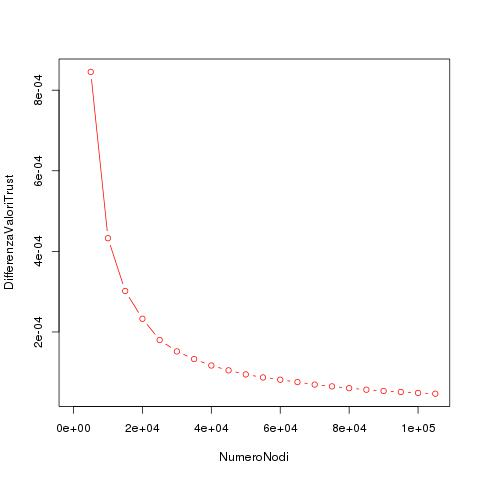
\includegraphics[height=9cm]{immagini/test5/averageTest_trust_112}
  \caption{Test 5 (trustrank,112). Differenza tra le medie dei valori di trustrank, calcolati sul grafo temporaneo ottenuto ad ogni intervallo di nodi visitati tramite la visita in ampiezza con nodo sorgente 112, dei nodi non spam e nodi spam.}
 \label{fig:test5trust112}
\end{figure}

In figura \ref{fig:test5trust62} e in figura \ref{fig:test5trust112} sono illustrate rispettivamente le differenze \(Diff_t\) la prima calcolata attreso una visita in ampiezza con nodo sorgete 62 mentre la seconda la visita in ampiezza ha nodo sorgente 112. Il risultato dei grafici è un po' inaspettato in quanto all'inzio della visita la differenza delle medie dei valori di \textit{trustrank} tra i nodi non spam e i nodi spam, calcolati sul grafo temporaneo, ha un valore più alto rispetto alla differenza delle medie dei valori di \textit{trustrnk} tra i nodi non spam e i nodi spam, calcolati sul grafo temporaneo che si ottiene ai successivi passi della visita in ampiezza. Questo significa che la distanza tra i valori di \textit{trustrank} tra i nodi non spam e spam tende ad essere meno marcata quando \textit{trustrank} viene calcolato sul grafo temporaneo composto da quasi tutti i nodi dell'intero grafo (infatti la curva tende a decrescerre).
Ma il comportamento che ci si aspettava, e che i grafici smentiscono, è che al momento del calcolo sul grafo ottenuto ai primi passi della visita i valori di \textit{trustrank} dei nodi non spam e spam avrebbero dovuto essere abbastanza vicini e quindi la diffenza tra la media \(Mb_t\) dei valori di \textit{trustrank} dei nodi non spam con la media \(Ms_t\) dei valori di \textit{trustrank} dei nodi spam dovrebbe essere abbastanza piccola. Ma verso la fine della visita, e quindi quando il grafo temporaneo è composto dalla maggior parte dei nodi dell'intero grafo, i valori di \textit{trustrank} dei nodi non spam e nodi spam dovrebbero essere molto distanti ovvero i nodi non spam dovrebbero avere avuto valori più alti di \textit{trustrank} (dal momento che \textit{trustrank} calcola un valore per ogni nodo di garazia che non si spam) rispetto ai nodi spam e la differenza tra la media \(Mb_t\) dei valori di \textit{trustrank} dei nodi non spam con la media \(Ms_t\) dei valori di \textit{trustrank} dei nodi spam 
dovrebbe essere molto grande in quanto \(Diff_t = Mb_t-Ms_t\) e \(Mb_t >> Ms_t\) e quindi i grafici in figura \ref{fig:test5trust62} e in figura \ref{fig:test5trust112} sarebbero dovuti essere crescenti.
\begin{figure}
 \centering
 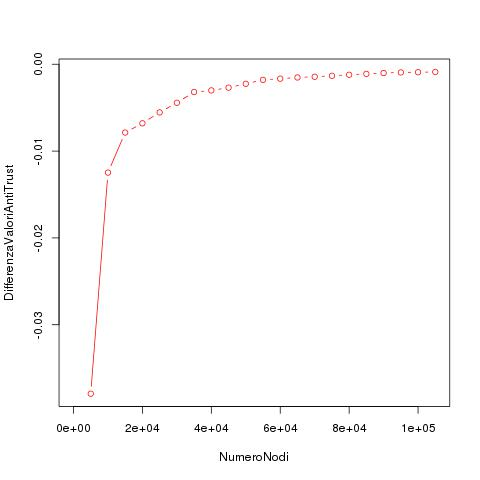
\includegraphics[height=9cm]{immagini/test5/averageTest_antitrust_62}
  \caption{Test 5 (anti-trust rank,62). Differenza tra le medie dei valori di antit-rust rank, calcolati sul grafo temporaneo ottenuto ad ogni intervallo di nodi visitati tramite la visita in ampiezza con nodo sorgente 62, dei nodi non spam e nodi spam.}
 \label{fig:test5antitrust62}
  \centering
 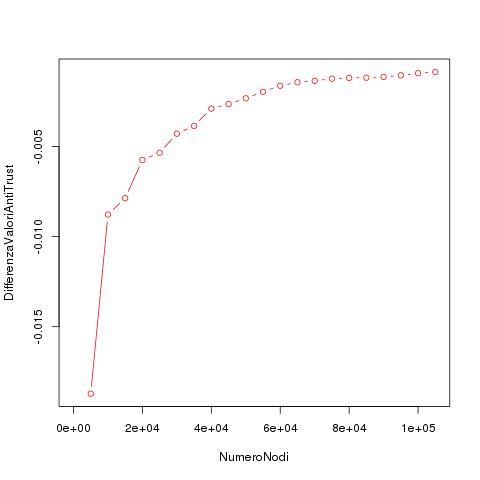
\includegraphics[height=9cm]{immagini/test5/averageTest_antitrust_112}
  \caption{Test 5 (anti-trust rank,112). Differenza tra le medie dei valori di anti-trust rank, calcolati sul grafo temporaneo ottenuto ad ogni intervallo di nodi visitati tramite la visita in ampiezza con nodo sorgente 112, dei nodi non spam e nodi spam.}
 \label{fig:test5antitrust112}
\end{figure}

In figura \ref{fig:test5antitrust62} e in figura \ref{fig:test5antitrust112} sono illustrati i grafici relativi alla differenza tra la differenza \(Diff_a\) tra le media \(Mb_a\) dei valori di \textit{anti-trust rank}, calcolati sul grafo temporaneo ottenuto ad ogni intervallo di nodi visitati tramite un visita in ampiezza, dei nodi non spam ,e la media \(Ms_a\) dei valori di \textit{anti-trust rank}, calcolati sul grafo temporaneo ottenuto ad ogni intervallo di nodi visitati tramite un visita in ampiezza, dei nodi etichettati spam. Nel primo grafico il nodo sorgente della visita in ampiezza è 62 nel secondo è 112. Anche in questo caso i risultati illustrati nei due grafici disapprovano le nostre attese in quanto il valore di \(Diff_a\) aumenta con l'aumentare dei nodi del grafo temporaneo su cui viene calcolato \(\hat{a}_i\). Tale risutato indica che il calcolo di \(\hat{a}_i\) sul grafo temporaneo ottenuto ai primi passi della visita (e quindi con pochi nodi) discrimina più fortemente i nodi non spam da 
quelli spam, in quanto la differenza \(Diff_a\) è molto piccola, rispetto al calcolo di \(\hat{a}_i\) sul grafo temporaneo ottenuto al termine della visita (e quidi quando rispecchia quasi totalemnte il grafo completo) dove i valori di \(\hat{a}_i\) sono meno distanti tra i nodi non spam e spam, in quanto la differenza \(Diff_a\) è molto più grande.\\
Differentemente da quanto descritto per \textit{trustrank} nel caso di \textit{anti-trust rank} ci si aspetta (ma i grafici smentiscono) che \(\hat{a}_i\) calcolato all'inzio della visita restituisca dei valori per i nodi non spam e per i nodi spam molto vicini e, quindi \(Diff_a\) sarebbe dovuta essere molto piccola prossima a 0, mentre  \(\hat{a}_i\) calcolato verso la fine della visita restituisca dei valori per i nodi non spam molto piccoli (perché \textit{anti-trust rank} indica il punteggio di spam di un nodo differentemente da \textit{trustrank} che indica il punteggio di garanzia un nodo sia non spam) e per i nodi spam dei valori molto alti e quindi \(Diff_a\) sarebbe dovuta essere negativa in quanto \( Diff_a=Mb_a-Ms_a\) e \(Mb_a << Ms_a\). Quindi i grafici in figura \ref{fig:test5antitrust62} e in figura \ref{fig:test5antitrust112} avrebbero dovuto avere una curva decrescente anziche crescente ovvero avrebbero dovuto avere un andamento inverso a quello illustrato. 

\section{Test 6}
Questo test è stato ideato per giustificare i dati ottenuti nel \textit{test numero 5}. Il test consiste nell'esecuzione di una visita in ampiezza \(v\) sul grafo \(G\) del dataset preso in esame con nodo sorgente \(s\) (dove il nodo sorgente è 62 e poi 112) e per ogni intervallo di nodi visitati si ricava il grafo temporaneo \(G_v\). Quindi si determinano i nodi etichettati non spam e spam del grafo temporaneo e utilizzando il loro valore di \textit{trustrank}  (o \textit{anti-trust rank}) calcolato sull'intero grafo \(G\) si calcola la differenza \(Diff_t\) (o \(Diff_a\) nel caso di \textit{anti-trust rank}) tra la media \(Mb_t\) nel caso di \textit{trustrank}, \(Mb_a\) nel caso di \textit{anti-trust rank}, dei valori dei nodi non spam e la media \(Ms_t\) nel caso di \textit{trustrank}, \(Ms_a\) nel caso di \textit{anti-trust rank}, dei valori dei nodi spam. Perciò si vuole vedere se i risultati del \textit{test numero 5} dipendono dai valori calcolati sull'intero grafo \(G\) di \textit{trustrank} e \textit{anti-trust rank}.
\begin{figure}
 \centering
 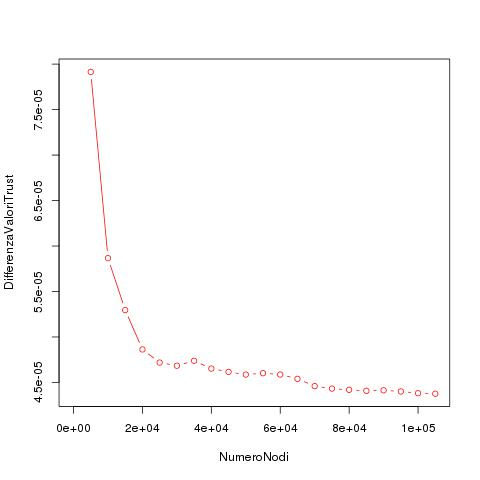
\includegraphics[height=9cm]{immagini/test6/averageCompleteTest_trust_62}
  \caption{Test 6 (trustrank,62). Differenza tra la media dei valori di trustrank finali dei nodi non spam e la media dei valori di trustrank nodi spam, per ogni intervallo di nodi visitati tramite la visita in ampiezza con nodo sorgente 62.}
 \label{fig:test6trust62}
  \centering
 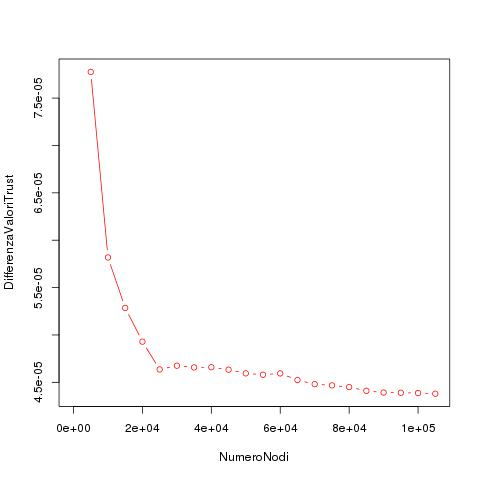
\includegraphics[height=9cm]{immagini/test6/averageCompleteTest_trust_112}
  \caption{Test 5 (trustrank,112). Differenza tra la media dei valori di trustrank finali dei nodi non spam e la media dei valori di trustrank nodi spam, per ogni intervallo di nodi visitati tramite la visita in ampiezza con nodo sorgente 112.}
 \label{fig:test6trust112}
\end{figure} 
In figura \ref{fig:test6trust62} è illustrato il grafico del calcolo di \(Diff_t\) dove il nodo sorgente della visita in ampiezza è 62 mentre in figura \ref{fig:test6trust112} è illustrato il grafico del calcolo di \(Diff_t\) dove il nodo sorgente della visita in ampiezza è 112. In entrambi i grafici sull'asse delle ascisse è rappresentato il numero di nodi visitati tramite la visita in ampiezza mentre sull'asse delle ordinate è rappresentata \(Diff_t\) calcolata ad ogni intervallo di nodi visitato attraverso la visita in ampiezza. L'andamento dei grafici giustica i risultati ottenuti per il \textit{test numero 5} in figura \ref{fig:test5trust62} e in figura \ref{fig:test5trust112}. Infatti l'andamento dei due grafici è simile ma cambia solamente la grandezza del range in cui varia \(Diff_t\) dove nel \textit{test numeto 5} il range è maggiore. Tale fatto spiega che i valori di \textit{trustrank} dei gruppo di nodi spam e non spam, contrariamente a quanto ci si aspetta, sono molto vicini ed invece sono molto più distanti i valori di \textit{trustrank} temporanei dei due gruppo di nodi calcolati sui grafi ottenuti all'inzio della visita in ampiezza. 

In figura \ref{fig:test6antitrust62}  è illustrato il grafico del calcolo di \(Diff_a\) dove il nodo sorgente della visita in ampiezza è 62 mentre in figura \ref{fig:test6antitrust112} è illustrato il grafico del calcolo di \(Diff_a\) dove il nodo sorgente della visita in ampiezza è 112. In entrambi i grafici sull'asse delle ascisse è rappresentato il numero di nodi visitati tramite la visita in ampiezza mentre sull'asse delle ordinate è rappresentata \(Diff_a\) calcolata ad ogni intervallo di nodi visitato attraverso la visita in ampiezza. Si nota che \(Diff_a\) calcolato all'inizio della visita usando i valori finali e \(Diff_a\) calcolato alla fine della visita usanto i valori finali siano molto vicini, nel primo grafico vi è uno  scarto di circa 0.00008 mentre nel secondo di circa 0.00006. Quindi indica che i risultati ottenuti nel \textit{test numeto 5} sono giusti ovvero che alla fine della visita la separazione dei valori di \textit{anti-trust rank} tra il gruppo di nodi spam e quelli non spam è meno marcata.
\begin{figure}
 \centering
 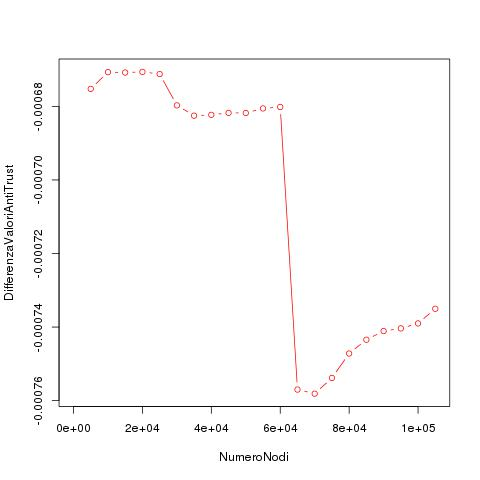
\includegraphics[height=9cm]{immagini/test6/averageCompleteTest_antitrust_62}
  \caption{Test 6 (trustrank,62). Differenza tra la media dei valori di trustrank finali dei nodi non spam e la media dei valori di trustrank nodi spam, per ogni intervallo di nodi visitati tramite la visita in ampiezza con nodo sorgente 62.}
 \label{fig:test6antitrust62}
  \centering
 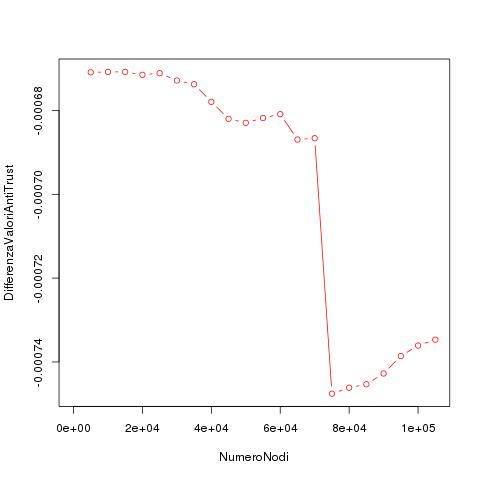
\includegraphics[height=9cm]{immagini/test6/averageCompleteTest_antitrust_112}
  \caption{Test 5 (trustrank,112). Differenza tra la media dei valori di trustrank finali dei nodi non spam e la media dei valori di trustrank nodi spam, per ogni intervallo di nodi visitati tramite la visita in ampiezza con nodo sorgente 112.}
 \label{fig:test6antitrust112}
\end{figure} 

\chapter{Conclusioni}

Col crescere delle dimensioni del web, aumenta la difficoltà di una pagina di comparire tra i primi risultati di un motore di ricerca per una data quey. Questo fenomeno porta allo sviluppo di meccanismi di spam per manipolare gli algoritmi dei motori di ricerca al fine di ottenere un rank maggiore per una data pagina web. Per combattere questi meccanismi di spam sono state introdotte varie tecniche di spam detection, la maggior parte delle quali operanti offline.\\
L'obbiettivo di questa tesi è stato, dunque, analizzare le  varie tecniche di spam detection descritte in letteratura al fine di analizzarne  il comportamento e vagliare la possibilità di utilizzo di tali tecnhiche online. 

Le varie tecniche descritte in letteratura sono state classificate in macro gruppi sulla base del tipo di segnale utilizzato; si sono individuati tre gruppi:
\begin{itemize}
 \item tecniche basate sul contenuto;
 \item tecniche basate sul grafo del web;
 \item tecniche innovative che usano segnali differenti dalle prime due. 
\end{itemize}
Le prime utilizzano il contenuto di una pagina web \(p\) per determinare se la pagina \(p\) è spam oppure non spam; le seconde utilizzano il grafo delle pagine web, ricavato dai link tra le pagine, per determinare se la pagina è spam o non spam; le terze, invece, utilizzano tipi di segnali eterogenei per identificare la natura di una pagina web \(p\) (ad esempio analizzando specifici pattern comportamentali dell'utente).

Dalla fase di analisi delle tecniche presenti in letteratura si è evinto che le tecniche di spam detection basate sul contenuto e sul grafo sono quelle più studiate e utilizzate. I metodi di spam detection innovativi che utilizzano segnali eterogenei sono poco studiati ma riescono ad identificare tipi di spam che i metodi classifici non rilevano; all'interno di questo insieme i metodi che fanno uso di pattern comportamentali rendono il problema dell’identificazione dello spam scalabile, ovvero consentono di rilevare nuove tipologie di spam web senza ogni volta definire nuove feature. Questo indica che tali metodi protrebbero essere utilizzati singolarmente mantenendo delle buone prestazioni. 
Al termine del lavoro di analisi è emerso quindi che l'utilizzo complementare dei metodi classici (basati sul contenuto e basati sul grafo) e dei metodi innovativi è ottimale per l' identificazine di pagine spam, in modo tale da raffinare la rilevazione di tali pagine.

Al termine della fase di documentazione si è deciso di analizzare due algoritmi di spam detection operanti offline, quali \textit{TrustRank} e \textit{Anti-Trust Rank} durante la fase di crawling. Il razionale di tale analisi è stato quindi la valutazione dell'operabilita di tali algoritmi durante l'esecuzione online e il confronto delle prestazioni rispetto all'utilizzo convenzionale offline.

Dai test condotti si è evinto che \textit{TrustRank} e \textit{Anti-Trust rank} online approssimano abbastanza bene il loro comportamento offline. Nello specifico le prestazioni dipendono dalla dimensione del grafo, derivato dalla fase di crawling, su cui vengono eseguiti i test. Tali deduzioni derivano dal fatto che la distanza tra il vettore di \textit{trustrank} ricavato offline è il vettore di \textit{TrustRank} ricavato durante la l'esecuzione online, diminuisce con l'aumentare della dimensione del grafo temporaneo su cui viene calcolato \textit{TrustRank} online (\textit{test numero 1}). Le stesse considerazioni valgono per \textit{Anti-Trust Rank}. Inoltre i risultati dei test  indicano che fin dall'inizio del crawling le prestazioni degli algoritmi in modalità online sono abbastanza affidabili, infatti i valori delle Tau di Kendall applicate tra il vettore ottenuto in modalità online, nelle prime fasi del crawling, con il vettore ottenuto in modalità offline, sono abbastanza alti; in particolare nel \textit{Test numero 1} la Tau di Kendall all'inizio della visita,  nell'esame di \textit{TrustRank}, ha valore iniziale 0.7, e nell'esame di \textit{Anti-Trust Rank}, ha  valore iniziale 0.75. Questo implica che la distanza tra i due vettori all'inizio del crawling è molto piccola. Quindi è facile dedurre che questi due algoritmi di spam detection possano essere usati online.

Confrontando i due algoritmi si è evinto che \textit{Anti-Trust Rank} approssima, per quasi tutta la durata del crawling, meglio il comportamento offline e quindi è più indicato per essere usato durante la fase di crawling. Ma i due algoritmi invertono le loro prestazioni al termine del crawling, quando il grafo temporaneo è molto simile al grafo completo ottenuto offline.

Un modo di utilizzare questi algoritmi online sarebbe quello di basarsi sull'isolamento approssimato dell'insieme delle pagine buone. Dal momento che le pagine non spam difficilmente avranno link verso pagine spam, si protrebbero utilizzare gli algoritmi di \textit{TrustRank} e \textit{Anti-Trust Rank} in modalità online per identificare le pagine spam durante il crawling e quindi un volta identificati i nodi spam penalizzare questi e quelli che hanno dei link verso tali nodi; una soluzione estrema potrebbe essere di eliminare tutte le pagine appartenenti ad un nodo identificato come spam.

Quindi dalle conclusioni della fase di testing risulta vantaggioso utilizzare questi algoritmi in modalità online avendo fin dall'inizio del crawling delle buone perfomance, inoltre una volta identificate le pagine spam molte altre pagine potrebbero essere non scaricate e quindi si eseguirebbero dei calcoli su grafi molto più piccoli e quindi usando minori risorse computazionali e di memorizzazione.

Sviluppo futuro di tale lavoro sarà la progettazione di un modulo di spam detection da inserire all'interno del  web crawler \textit{BUbiNG}, sviluppato dal Laboratorio di Algoritmica per il Web dell'Università degli Studi di Milano.



\backmatter
\bibliographystyle{ieeetr}
\bibliography{biblio,biblio2,biblio3,biblio4}
\end{document}
